\documentclass[]{book}
\usepackage{lmodern}
\usepackage{amssymb,amsmath}
\usepackage{ifxetex,ifluatex}
\usepackage{fixltx2e} % provides \textsubscript
\ifnum 0\ifxetex 1\fi\ifluatex 1\fi=0 % if pdftex
  \usepackage[T1]{fontenc}
  \usepackage[utf8]{inputenc}
\else % if luatex or xelatex
  \ifxetex
    \usepackage{mathspec}
  \else
    \usepackage{fontspec}
  \fi
  \defaultfontfeatures{Ligatures=TeX,Scale=MatchLowercase}
  \newcommand{\euro}{€}
\fi
% use upquote if available, for straight quotes in verbatim environments
\IfFileExists{upquote.sty}{\usepackage{upquote}}{}
% use microtype if available
\IfFileExists{microtype.sty}{%
\usepackage{microtype}
\UseMicrotypeSet[protrusion]{basicmath} % disable protrusion for tt fonts
}{}
\usepackage[margin=1in]{geometry}
\usepackage{hyperref}
\PassOptionsToPackage{usenames,dvipsnames}{color} % color is loaded by hyperref
\hypersetup{unicode=true,
            pdftitle={Advanced Visualisation and Data Wrangling in R},
            pdfauthor={TJ McKinley},
            colorlinks=true,
            linkcolor=blue,
            citecolor=Blue,
            urlcolor=Blue,
            breaklinks=true}
\urlstyle{same}  % don't use monospace font for urls
\usepackage{color}
\usepackage{fancyvrb}
\newcommand{\VerbBar}{|}
\newcommand{\VERB}{\Verb[commandchars=\\\{\}]}
\DefineVerbatimEnvironment{Highlighting}{Verbatim}{commandchars=\\\{\}}
% Add ',fontsize=\small' for more characters per line
\usepackage{framed}
\definecolor{shadecolor}{RGB}{248,248,248}
\newenvironment{Shaded}{\begin{snugshade}}{\end{snugshade}}
\newcommand{\KeywordTok}[1]{\textcolor[rgb]{0.13,0.29,0.53}{\textbf{{#1}}}}
\newcommand{\DataTypeTok}[1]{\textcolor[rgb]{0.13,0.29,0.53}{{#1}}}
\newcommand{\DecValTok}[1]{\textcolor[rgb]{0.00,0.00,0.81}{{#1}}}
\newcommand{\BaseNTok}[1]{\textcolor[rgb]{0.00,0.00,0.81}{{#1}}}
\newcommand{\FloatTok}[1]{\textcolor[rgb]{0.00,0.00,0.81}{{#1}}}
\newcommand{\ConstantTok}[1]{\textcolor[rgb]{0.00,0.00,0.00}{{#1}}}
\newcommand{\CharTok}[1]{\textcolor[rgb]{0.31,0.60,0.02}{{#1}}}
\newcommand{\SpecialCharTok}[1]{\textcolor[rgb]{0.00,0.00,0.00}{{#1}}}
\newcommand{\StringTok}[1]{\textcolor[rgb]{0.31,0.60,0.02}{{#1}}}
\newcommand{\VerbatimStringTok}[1]{\textcolor[rgb]{0.31,0.60,0.02}{{#1}}}
\newcommand{\SpecialStringTok}[1]{\textcolor[rgb]{0.31,0.60,0.02}{{#1}}}
\newcommand{\ImportTok}[1]{{#1}}
\newcommand{\CommentTok}[1]{\textcolor[rgb]{0.56,0.35,0.01}{\textit{{#1}}}}
\newcommand{\DocumentationTok}[1]{\textcolor[rgb]{0.56,0.35,0.01}{\textbf{\textit{{#1}}}}}
\newcommand{\AnnotationTok}[1]{\textcolor[rgb]{0.56,0.35,0.01}{\textbf{\textit{{#1}}}}}
\newcommand{\CommentVarTok}[1]{\textcolor[rgb]{0.56,0.35,0.01}{\textbf{\textit{{#1}}}}}
\newcommand{\OtherTok}[1]{\textcolor[rgb]{0.56,0.35,0.01}{{#1}}}
\newcommand{\FunctionTok}[1]{\textcolor[rgb]{0.00,0.00,0.00}{{#1}}}
\newcommand{\VariableTok}[1]{\textcolor[rgb]{0.00,0.00,0.00}{{#1}}}
\newcommand{\ControlFlowTok}[1]{\textcolor[rgb]{0.13,0.29,0.53}{\textbf{{#1}}}}
\newcommand{\OperatorTok}[1]{\textcolor[rgb]{0.81,0.36,0.00}{\textbf{{#1}}}}
\newcommand{\BuiltInTok}[1]{{#1}}
\newcommand{\ExtensionTok}[1]{{#1}}
\newcommand{\PreprocessorTok}[1]{\textcolor[rgb]{0.56,0.35,0.01}{\textit{{#1}}}}
\newcommand{\AttributeTok}[1]{\textcolor[rgb]{0.77,0.63,0.00}{{#1}}}
\newcommand{\RegionMarkerTok}[1]{{#1}}
\newcommand{\InformationTok}[1]{\textcolor[rgb]{0.56,0.35,0.01}{\textbf{\textit{{#1}}}}}
\newcommand{\WarningTok}[1]{\textcolor[rgb]{0.56,0.35,0.01}{\textbf{\textit{{#1}}}}}
\newcommand{\AlertTok}[1]{\textcolor[rgb]{0.94,0.16,0.16}{{#1}}}
\newcommand{\ErrorTok}[1]{\textcolor[rgb]{0.64,0.00,0.00}{\textbf{{#1}}}}
\newcommand{\NormalTok}[1]{{#1}}
\usepackage{longtable,booktabs}
\usepackage{graphicx,grffile}
\makeatletter
\def\maxwidth{\ifdim\Gin@nat@width>\linewidth\linewidth\else\Gin@nat@width\fi}
\def\maxheight{\ifdim\Gin@nat@height>\textheight\textheight\else\Gin@nat@height\fi}
\makeatother
% Scale images if necessary, so that they will not overflow the page
% margins by default, and it is still possible to overwrite the defaults
% using explicit options in \includegraphics[width, height, ...]{}
\setkeys{Gin}{width=\maxwidth,height=\maxheight,keepaspectratio}
\setlength{\parindent}{0pt}
\setlength{\parskip}{6pt plus 2pt minus 1pt}
\setlength{\emergencystretch}{3em}  % prevent overfull lines
\providecommand{\tightlist}{%
  \setlength{\itemsep}{0pt}\setlength{\parskip}{0pt}}
\setcounter{secnumdepth}{5}

%%% Use protect on footnotes to avoid problems with footnotes in titles
\let\rmarkdownfootnote\footnote%
\def\footnote{\protect\rmarkdownfootnote}

%%% Change title format to be more compact
\usepackage{titling}

% Create subtitle command for use in maketitle
\newcommand{\subtitle}[1]{
  \posttitle{
    \begin{center}\large#1\end{center}
    }
}

\setlength{\droptitle}{-2em}

  \title{Advanced Visualisation and Data Wrangling in R}
    \pretitle{\vspace{\droptitle}\centering\huge}
  \posttitle{\par}
    \author{TJ McKinley}
    \preauthor{\centering\large\emph}
  \postauthor{\par}
    \date{}
    \predate{}\postdate{}
  

% Redefines (sub)paragraphs to behave more like sections
\ifx\paragraph\undefined\else
\let\oldparagraph\paragraph
\renewcommand{\paragraph}[1]{\oldparagraph{#1}\mbox{}}
\fi
\ifx\subparagraph\undefined\else
\let\oldsubparagraph\subparagraph
\renewcommand{\subparagraph}[1]{\oldsubparagraph{#1}\mbox{}}
\fi

% latex macro to create task boxes
\usepackage{tcolorbox}

\definecolor{taskCol}{HTML}{404040}
\definecolor{taskCol1}{HTML}{808080}

\tcbset{colback=white,colframe=taskCol,arc=0mm}

%trick to fool markdown into compiling
\newcommand{\bblockT}[1]{\begin{tcolorbox}[title = Task #1]}
\newcommand{\eblockT}{\end{tcolorbox}}
\newcommand{\bblockS}[1]{\begin{tcolorbox}[title = Solution #1, colframe=taskCol1]}
\newcommand{\eblockS}{\end{tcolorbox}}

%set solution button link
\usepackage{tikz}

\newcommand{\buttonT}[1]{
    \begin{tikzpicture}
    \node[
        inner sep=5pt,
        draw=taskCol,
        fill=taskCol,
        rounded corners=2pt,
        text=white
    ] (c1) {#1};
    \end{tikzpicture}
}

\newcommand{\buttonS}[1]{
    \begin{tikzpicture}
    \node[
        inner sep=5pt,
        draw=taskCol1,
        fill=taskCol1,
        rounded corners=2pt,
        text=white
    ] (c1) {#1};
    \end{tikzpicture}
}

\usepackage{amsthm}
\newtheorem{theorem}{Theorem}[chapter]
\newtheorem{lemma}{Lemma}[chapter]
\theoremstyle{definition}
\newtheorem{definition}{Definition}[chapter]
\newtheorem{corollary}{Corollary}[chapter]
\newtheorem{proposition}{Proposition}[chapter]
\theoremstyle{definition}
\newtheorem{example}{Example}[chapter]
\theoremstyle{definition}
\newtheorem{exercise}{Exercise}[chapter]
\theoremstyle{remark}
\newtheorem*{remark}{Remark}
\newtheorem*{solution}{Solution}
\begin{document}
\maketitle

{
\hypersetup{linkcolor=black}
\setcounter{tocdepth}{1}
\tableofcontents
}
\chapter*{Introduction}\label{introduction}
\addcontentsline{toc}{chapter}{Introduction}

This workshop requires that you're comfortable with R, and specifically
with the concept of \texttt{data.frame} objects. The ability to work
with and visualise data frames is one of the key reasons why R is so
popular amongst statisticians and data scientists. Although a vast
amount can be achieved using base R functionality, one of R's other key
strengths is the vast array of
\href{https://cran.r-project.org/web/packages/}{packages} that it
supports, which add a rich variety of additional functionality to R.

A suite of packages that are fast becoming \emph{de rigueur} for
performing myriad data science tasks is known as the
\href{https://www.tidyverse.org/}{\texttt{tidyverse}}. These packages
provide powerful functions for doing visualisation and manipulation of
complex data sets. In this workshop we will introduce key
\texttt{tidyverse} packages, such as \texttt{readr}, \texttt{tidyr},
\texttt{dplyr} and \texttt{ggplot2}, and show how they can be used to
efficiently process and visualise complex data.

\section*{\texorpdfstring{\texttt{tidyverse}
packages}{tidyverse packages}}\label{tidyverse-packages}
\addcontentsline{toc}{section}{\texttt{tidyverse} packages}

The \href{https://www.tidyverse.org/}{\texttt{tidyverse}} is a suite of
packages, including \texttt{tidyr}, \texttt{dplyr}, \texttt{ggplot2},
\texttt{purrr}, \texttt{tibble} and \texttt{readr}. Although these
packages can each be installed and loaded separately, they are designed
to work together, and as such will simply install and load the
\texttt{tidyverse} directly, rather than worry too much about which
functions belong to which packages.

To install \texttt{tidyverse}, use:

\begin{Shaded}
\begin{Highlighting}[]
\KeywordTok{install.packages}\NormalTok{(}\StringTok{"tidyverse"}\NormalTok{)}
\end{Highlighting}
\end{Shaded}

and once installed, it can be loaded using:

\begin{Shaded}
\begin{Highlighting}[]
\KeywordTok{library}\NormalTok{(tidyverse)}
\end{Highlighting}
\end{Shaded}

in the usual way.

\begin{quote}
\textbf{Note}: if you are loading \texttt{tidyverse} as part of an R
Markdown document, and you want to knit to a PDF document using
\(\LaTeX\), then it sometimes throws an error when loading because
\(\LaTeX\) can't process the correct fonts for the loading message.
Hence in R Markdown documents I always suppress the load messages
through the chunk option \texttt{message\ =\ F} e.g.

\begin{verbatim}
```{r, message = F}
library(tidyverse)
```
\end{verbatim}
\end{quote}

\section*{Tasks}\label{tasks}
\addcontentsline{toc}{section}{Tasks}

\hypertarget{tsk1}{}\bblockT{1}

All \textbf{tasks} will be denoted in panel boxes like this one. In the
HTML version, all solutions can be toggled by hitting the \textbf{Show
Solution} buttons. In the PDF version solutions are given in the
Appendix and are linked via the \textbf{Show Solution} buttons. \eblockT

\hyperlink{sol1}{\buttonS{Show Solution}}

\chapter{\texorpdfstring{Visualisation using
\texttt{ggplot2}}{Visualisation using ggplot2}}\label{visualisation-using-ggplot2}

Let's start with a motivating example.

\section{Gapminder}\label{gapminder}

\href{https://en.wikipedia.org/wiki/Hans_Rosling}{Professor Hans
Rosling} has made a name for himself in the field of data visualisation
with his groundbreaking \href{https://www.gapminder.org/}{Gapminder}
project.

\begin{center}\includegraphics{images/hans} \end{center}

For a slightly longer presentation, his TED talk on global development
has been watched over 11 million times. If you have 20 minutes, it can
be found
\href{https://www.ted.com/talks/hans_rosling_shows_the_best_stats_you_ve_ever_seen?utm_source=tedcomshare\&utm_medium=referral\&utm_campaign=tedspread}{here},
and is well worth a watch!

\begin{quote}
More-or-less as I had finished the first version of these notes, the
news broke that Professor Rosling had sadly passed away on 7th February
2017, aged 68. I hope you will find some time to explore the
\href{https://www.gapminder.org/}{Gapminder} website, and appreciate the
immense contribution that he made to the world of public health and
education. He presented a world-view based on facts and data. To this
end he provided innovative and fascinating ways to explore and
understand data, disseminated these findings with pathos and humour, and
used this information to challenge many of our pre-conceptions about
public health and the developing world. An obituary from the Guardian
can be found
\href{https://www.theguardian.com/global-development/2017/feb/07/hans-rosling-obituary}{here}.
\end{quote}

The \href{https://www.gapminder.org/}{Gapminder} website provides really
informative interactive visualisations for many fascinating data sets.
In this pracical we will explore how to use R to try to recreate
something similar to the types of visualisation that Gapminder provides,
and see how high-end R packages---such as \texttt{ggplot2}---have been
developed that provide a systematic and flexible way to generate complex
plots / visualisations. Our aim for this workshop is to emulate the plot
in Figure \ref{fig:gapminder}.

\begin{figure}

{\centering \includegraphics{images/gapminder} 

}

\caption{Life expectancy against GDP---screenshot from Gapminder project}\label{fig:gapminder}
\end{figure}

Before we do this, let's quickly remind ourselves of basic plotting
functionality in R.

\section{Base R graphics}\label{base-r-graphics}

Let's begin by exploring the \texttt{iris} data set, which gives the
measurements in centimeters of the variables sepal length and width, and
petal length and width, respectively, for 50 flowers from each of 3
species of iris. The species are \emph{Iris setosa}, \emph{versicolor},
and \emph{virginica}. This data set is available as part of the base R
package. Let's have a look at the data:

\begin{Shaded}
\begin{Highlighting}[]
\KeywordTok{head}\NormalTok{(iris)}
\end{Highlighting}
\end{Shaded}

\begin{verbatim}
##   Sepal.Length Sepal.Width Petal.Length Petal.Width Species
## 1          5.1         3.5          1.4         0.2  setosa
## 2          4.9         3.0          1.4         0.2  setosa
## 3          4.7         3.2          1.3         0.2  setosa
## 4          4.6         3.1          1.5         0.2  setosa
## 5          5.0         3.6          1.4         0.2  setosa
## 6          5.4         3.9          1.7         0.4  setosa
\end{verbatim}

Let's start by visualising the variable \texttt{Sepal.Length}using a
kernel density plot:.

\begin{Shaded}
\begin{Highlighting}[]
\NormalTok{## kernel density of sepal length}
\KeywordTok{plot}\NormalTok{(}\KeywordTok{density}\NormalTok{(iris$Sepal.Length))}
\end{Highlighting}
\end{Shaded}

\begin{center}\includegraphics{_main_files/figure-latex/unnamed-chunk-8-1} \end{center}

\begin{quote}
Remember that we can extract a named column from a \texttt{data.frame}
using the \texttt{\$} operator. The \texttt{density()} function is a
simple function in R that takes a \texttt{vector} argument and returns a
kernel density object, which we can then plot using the generic
\texttt{plot()} function.
\end{quote}

Now let's try to plot different kernel density plots for the three
different species. We could do this as separate plots, and use our
standard subsetting notation to extract the correct elements of the data
frame in each case:

\begin{Shaded}
\begin{Highlighting}[]
\NormalTok{## plot Sepal.Length for setosa}
\KeywordTok{plot}\NormalTok{(}\KeywordTok{density}\NormalTok{(iris$Sepal.Length[iris$Species ==}\StringTok{ "setosa"}\NormalTok{]))}

\NormalTok{## plot Sepal.Length for versicolor}
\KeywordTok{plot}\NormalTok{(}\KeywordTok{density}\NormalTok{(iris$Sepal.Length[iris$Species ==}\StringTok{ "versicolor"}\NormalTok{]))}

\NormalTok{## plot Sepal.Length for virginica}
\KeywordTok{plot}\NormalTok{(}\KeywordTok{density}\NormalTok{(iris$Sepal.Length[iris$Species ==}\StringTok{ "virginica"}\NormalTok{]))}
\end{Highlighting}
\end{Shaded}

\begin{center}\includegraphics{_main_files/figure-latex/unnamed-chunk-9-1} \includegraphics{_main_files/figure-latex/unnamed-chunk-9-2} \includegraphics{_main_files/figure-latex/unnamed-chunk-9-3} \end{center}

What about if we want to add all three histograms to the same plot?

\begin{Shaded}
\begin{Highlighting}[]
\NormalTok{## add two histograms to the same plot}
\KeywordTok{plot}\NormalTok{(}\KeywordTok{density}\NormalTok{(iris$Sepal.Length[iris$Species ==}\StringTok{ "setosa"}\NormalTok{]), }\DataTypeTok{main =} \StringTok{""}\NormalTok{)}
\KeywordTok{lines}\NormalTok{(}\KeywordTok{density}\NormalTok{(iris$Sepal.Length[iris$Species ==}\StringTok{ "versicolor"}\NormalTok{]))}
\KeywordTok{lines}\NormalTok{(}\KeywordTok{density}\NormalTok{(iris$Sepal.Length[iris$Species ==}\StringTok{ "virginica"}\NormalTok{]))}
\end{Highlighting}
\end{Shaded}

\begin{center}\includegraphics{_main_files/figure-latex/unnamed-chunk-10-1} \end{center}

\begin{quote}
Notice the use of the \texttt{lines()} function to allow a line to be
added to an existing plot.
\end{quote}

Notice that the limits of the \(x\)- and \(y\)-axes in this case are set
by the range of the initial \texttt{setosa} sepal lengths, and hence the
density plots for the other two species extend beyond the plot window.
Let's try again, but this time setting the bounds for the plots
manually. To do this we calculate the \(x\) and \(y\) ranges for each
density plot separately, and then take the maximum values across the
different species. We then use the \texttt{xlim} and \texttt{ylim}
arguments to the \texttt{plot()} function in order to set the ranges:

\begin{Shaded}
\begin{Highlighting}[]
\NormalTok{## produce densities}
\NormalTok{setosa_dens <-}\StringTok{ }\KeywordTok{density}\NormalTok{(iris$Sepal.Length[iris$Species ==}\StringTok{ "setosa"}\NormalTok{])}
\NormalTok{versicolor_dens <-}\StringTok{ }\KeywordTok{density}\NormalTok{(iris$Sepal.Length[iris$Species ==}\StringTok{ "versicolor"}\NormalTok{])}
\NormalTok{virginica_dens <-}\StringTok{ }\KeywordTok{density}\NormalTok{(iris$Sepal.Length[iris$Species ==}\StringTok{ "virginica"}\NormalTok{])}

\NormalTok{## extract x-ranges and y-ranges}
\NormalTok{xlims <-}\StringTok{ }\KeywordTok{range}\NormalTok{(}\KeywordTok{c}\NormalTok{(setosa_dens$x, versicolor_dens$x, virginica_dens$x))}
\NormalTok{ylims <-}\StringTok{ }\KeywordTok{range}\NormalTok{(}\KeywordTok{c}\NormalTok{(setosa_dens$y, versicolor_dens$y, virginica_dens$y))}

\NormalTok{## produce plot}
\KeywordTok{plot}\NormalTok{(}\KeywordTok{density}\NormalTok{(iris$Sepal.Length[iris$Species ==}\StringTok{ "setosa"}\NormalTok{]), }
     \DataTypeTok{xlim =} \NormalTok{xlims, }\DataTypeTok{ylim =} \NormalTok{ylims, }\DataTypeTok{main =} \StringTok{""}\NormalTok{)}
\KeywordTok{lines}\NormalTok{(}\KeywordTok{density}\NormalTok{(iris$Sepal.Length[iris$Species ==}\StringTok{ "versicolor"}\NormalTok{]))}
\KeywordTok{lines}\NormalTok{(}\KeywordTok{density}\NormalTok{(iris$Sepal.Length[iris$Species ==}\StringTok{ "virginica"}\NormalTok{]))}
\end{Highlighting}
\end{Shaded}

\begin{center}\includegraphics{_main_files/figure-latex/unnamed-chunk-11-1} \end{center}

This is better, but still not very informative. Let's add some colour
and a legend, and tidy up the axis labels.

\begin{Shaded}
\begin{Highlighting}[]
\NormalTok{## produce plot}
\KeywordTok{plot}\NormalTok{(}\KeywordTok{density}\NormalTok{(iris$Sepal.Length[iris$Species ==}\StringTok{ "setosa"}\NormalTok{]), }
    \DataTypeTok{xlim =} \NormalTok{xlims, }\DataTypeTok{ylim =} \NormalTok{ylims, }\DataTypeTok{main =} \StringTok{""}\NormalTok{, }\DataTypeTok{xlab =} \StringTok{"Sepal Length (cm)"}\NormalTok{)}
\KeywordTok{lines}\NormalTok{(}\KeywordTok{density}\NormalTok{(iris$Sepal.Length[iris$Species ==}\StringTok{ "versicolor"}\NormalTok{]), }\DataTypeTok{col =} \StringTok{"red"}\NormalTok{)}
\KeywordTok{lines}\NormalTok{(}\KeywordTok{density}\NormalTok{(iris$Sepal.Length[iris$Species ==}\StringTok{ "virginica"}\NormalTok{]), }\DataTypeTok{col =} \StringTok{"blue"}\NormalTok{)}

\NormalTok{## add legend to top-right corner}
\KeywordTok{legend}\NormalTok{(}\KeywordTok{par}\NormalTok{(}\StringTok{"usr"}\NormalTok{)[}\DecValTok{2}\NormalTok{] *}\StringTok{ }\FloatTok{0.8}\NormalTok{, }\KeywordTok{par}\NormalTok{(}\StringTok{"usr"}\NormalTok{)[}\DecValTok{4}\NormalTok{] *}\StringTok{ }\FloatTok{0.95}\NormalTok{, }
       \DataTypeTok{legend =} \KeywordTok{c}\NormalTok{(}\StringTok{"setosa"}\NormalTok{, }\StringTok{"versicolor"}\NormalTok{, }\StringTok{"virginica"}\NormalTok{), }
       \DataTypeTok{lty =} \KeywordTok{c}\NormalTok{(}\DecValTok{1}\NormalTok{, }\DecValTok{1}\NormalTok{, }\DecValTok{1}\NormalTok{), }
       \DataTypeTok{col =} \KeywordTok{c}\NormalTok{(}\StringTok{"black"}\NormalTok{, }\StringTok{"red"}\NormalTok{, }\StringTok{"blue"}\NormalTok{))}
\end{Highlighting}
\end{Shaded}

\begin{center}\includegraphics{_main_files/figure-latex/unnamed-chunk-12-1} \end{center}

Notice that this is quite a simple plot, but required a series of steps
to render in base R. We needed to calculate manual limits for the axes,
plot the three species separately, and then add a custom legend to the
plot.

Let's look at another quick example. This time, let's plot sepal length
against sepal width for the three species.

\begin{Shaded}
\begin{Highlighting}[]
\NormalTok{## produce scatterplot}
\KeywordTok{plot}\NormalTok{(iris$Sepal.Length, iris$Sepal.Width, }
     \DataTypeTok{xlab =} \StringTok{"Sepal Length (cm)"}\NormalTok{, }\DataTypeTok{ylab =} \StringTok{"Sepal Width (cm)"}\NormalTok{)}
\KeywordTok{points}\NormalTok{(iris$Sepal.Length[iris$Species ==}\StringTok{ "versicolor"}\NormalTok{],}
       \NormalTok{iris$Sepal.Width[iris$Species ==}\StringTok{ "versicolor"}\NormalTok{], }\DataTypeTok{col =} \StringTok{"red"}\NormalTok{)}
\KeywordTok{points}\NormalTok{(iris$Sepal.Length[iris$Species ==}\StringTok{ "virginica"}\NormalTok{],}
       \NormalTok{iris$Sepal.Width[iris$Species ==}\StringTok{ "virginica"}\NormalTok{], }\DataTypeTok{col =} \StringTok{"blue"}\NormalTok{)}

\NormalTok{## add legend}
\KeywordTok{legend}\NormalTok{(}\KeywordTok{par}\NormalTok{(}\StringTok{"usr"}\NormalTok{)[}\DecValTok{2}\NormalTok{] *}\StringTok{ }\FloatTok{0.8}\NormalTok{, }\KeywordTok{par}\NormalTok{(}\StringTok{"usr"}\NormalTok{)[}\DecValTok{4}\NormalTok{] *}\StringTok{ }\FloatTok{0.98}\NormalTok{, }
       \DataTypeTok{legend =} \KeywordTok{c}\NormalTok{(}\StringTok{"setosa"}\NormalTok{, }\StringTok{"versicolor"}\NormalTok{, }\StringTok{"virginica"}\NormalTok{), }
       \DataTypeTok{pch =} \KeywordTok{c}\NormalTok{(}\DecValTok{1}\NormalTok{, }\DecValTok{1}\NormalTok{, }\DecValTok{1}\NormalTok{), }
       \DataTypeTok{col =} \KeywordTok{c}\NormalTok{(}\StringTok{"black"}\NormalTok{, }\StringTok{"red"}\NormalTok{, }\StringTok{"blue"}\NormalTok{))}
\end{Highlighting}
\end{Shaded}

\begin{center}\includegraphics{_main_files/figure-latex/unnamed-chunk-13-1} \end{center}

\begin{quote}
Notice the use of the \texttt{points()} function to add points to an
existing plot. We could set the position of the legend manually, but the
objects \texttt{par("usr")} provides the coordinates of the plot region
in the form \texttt{c(x1,\ x2,\ y1,\ y2)}, where \texttt{x1} is the
lower bound for the \(x\)-axis, and \texttt{x2} is the upper bound for
the \(x\)-axis, and similarly for \texttt{y1} and \texttt{y2}.
\end{quote}

\section{\texorpdfstring{Introduction to
\texttt{ggplot2}}{Introduction to ggplot2}}\label{introduction-to-ggplot2}

We have seen that the R base graphics system is highly flexible, and can
be used to produce high-quality, bespoke visualisations. However, it was
a lot of work! Let's show an alternative way to produce similar plots
using the \texttt{ggplot2} package. We will introduce the code first,
and then talk through it.

First we load the \texttt{tidyverse} (of which \texttt{ggplot2} is
included).

\begin{Shaded}
\begin{Highlighting}[]
\KeywordTok{library}\NormalTok{(tidyverse)}
\end{Highlighting}
\end{Shaded}

Now run

\begin{Shaded}
\begin{Highlighting}[]
\KeywordTok{ggplot}\NormalTok{(iris) +}
\StringTok{    }\KeywordTok{geom_point}\NormalTok{(}\KeywordTok{aes}\NormalTok{(}\DataTypeTok{x =} \NormalTok{Sepal.Length, }\DataTypeTok{y =} \NormalTok{Sepal.Width, }\DataTypeTok{colour =} \NormalTok{Species))}
\end{Highlighting}
\end{Shaded}

\begin{center}\includegraphics{_main_files/figure-latex/unnamed-chunk-15-1} \end{center}

Notice that we had to do little physical manipulation of the plot. We
didn't have to choose how to position legends, or manually subset the
data to plot the different points, or choose the colours; the package
took care of all of these things.

So, how does it work? \texttt{ggplot2} is based on a book called the
\href{https://www.amazon.co.uk/Grammar-Graphics-Statistics-Computing/dp/0387245448}{Grammar
of Graphics} by
\href{https://en.wikipedia.org/wiki/Leland_Wilkinson}{Leland
Wilkinson}---hence the name \texttt{gg}-\texttt{plot}! The ethos of
\texttt{ggplot2} is that plots can be broken down into different
\textbf{features}, most notably:

\begin{itemize}
\tightlist
\item
  \textbf{data};
\item
  \textbf{aesthetic mapping};
\item
  \textbf{geometric object};
\item
  \textbf{scales};
\item
  \textbf{faceting};
\item
  statistical transformations;
\item
  coordinate system;
\item
  position adjustments.
\end{itemize}

Perhaps the easiest way to explain some of these concepts is to work
through our examples step-by-step. We will focus on the main components
marked in \textbf{bold} above. Let's start with the scatterplot example
first, and examine the first part of the code:

\begin{Shaded}
\begin{Highlighting}[]
\KeywordTok{ggplot}\NormalTok{(iris)}
\end{Highlighting}
\end{Shaded}

\begin{center}\includegraphics{_main_files/figure-latex/unnamed-chunk-16-1} \end{center}

This sets up the plot. The first argument to the \texttt{ggplot}
function is the \textbf{data}, which here is the \texttt{iris} data set.

\begin{quote}
\textbf{Important}: whereas base R graphics can plot various object
types, \texttt{ggplot()} \textbf{requires} \texttt{data.frame} (or
\texttt{tibble}\footnote{We will see \texttt{tibble} objects later
  on---just think of them as special \texttt{data.frames}.}) objects. It
is designed for plotting statistical data sets. Never fear, most R
objects can be manipulated into \texttt{data.frames} for plotting if
required. (See next session on \textbf{data wrangling}.)
\end{quote}

\subsection{Aesthetics}\label{aesthetics}

The
\texttt{aes(x\ =\ Sepal.Length,\ y\ =\ Sepal.Width,\ colour\ =\ Species)}
part sets the \textbf{aesthetics}, which here are added as an argument
to the \texttt{geom\_point()} function (see nect section). These define
how the data are \textbf{mapped} onto the visual aesthetics of the plot.
Here we are setting the \texttt{x} coordinates to be
\texttt{Sepal.Length}, the \texttt{y} coordinates to be
\texttt{Sepal.Width}, and the \texttt{colour} of the characters to be
related to \texttt{Species}. In general, \textbf{aesthetics} include:

\begin{itemize}
\tightlist
\item
  position;
\item
  colour (border or line color);
\item
  fill (inside color);
\item
  shape;
\item
  linetype;
\item
  size.
\end{itemize}

\begin{quote}
As usual, information can be found in the relevant help files, but a
really useful resource for \texttt{ggplot2} is the
\href{https://github.com/rstudio/cheatsheets/raw/master/data-visualization-2.1.pdf}{Data
Visualisation Cheat Sheet}. Another fantastic resource, is the
\href{http://www.cookbook-r.com/Graphs/}{R Graphics Cookbook} by Winston
Chang, which has a free online version, or a physical book that you can
buy.
\end{quote}

\begin{quote}
\textbf{Notice} that we did not have to use the \texttt{\$} operator to
extract columns. This makes \texttt{ggplot2} code a lot clearer. R knows
to look for the \texttt{Sepal.Length} and \texttt{Sepal.Width} columns
in the \texttt{iris} data, because we have told \texttt{ggplot()} which
data set to operate on.
\end{quote}

\subsection{Geoms}\label{geoms}

\begin{quote}
A \textbf{geom} defines the type of plot we want. In this case we want a
\textbf{scatterplot}, which can be defined by the \texttt{geom\_point()}
function. Geoms can be layered, allowing us to built complex plots in
different ways. Common geoms are:

\begin{itemize}
\tightlist
\item
  \texttt{geom\_point()}
\item
  \texttt{geom\_line()}
\item
  \texttt{geom\_histogram()}
\item
  \texttt{geom\_density()}
\item
  \texttt{geom\_bar()}
\item
  \texttt{geom\_violin()}
\end{itemize}

Please see the
\href{https://github.com/rstudio/cheatsheets/raw/master/data-visualization-2.1.pdf}{Data
Visualisation Cheat Sheet} for more examples.
\end{quote}

\begin{quote}
\textbf{Note}: \texttt{ggplot2} \textbf{builds} plots up by
\emph{adding} together components. There are lots of ways to do this.
Here I have set up ``global'' options for the plot (including the
aesthetics) using the \texttt{ggplot()} function. I then \textbf{add}
(\texttt{+}) to this the type of plot I want i.e.
\texttt{+\ geom\_point()}. The addition sign is important. If I want to
split the function over multiple lines, make sure the \texttt{+} sign is
at the \textbf{end} of each line, so R knows that the plot is not
complete at the point.
\end{quote}

Let's see how this works:

\begin{Shaded}
\begin{Highlighting}[]
\KeywordTok{ggplot}\NormalTok{(iris) +}
\StringTok{    }\KeywordTok{geom_point}\NormalTok{(}\KeywordTok{aes}\NormalTok{(}\DataTypeTok{x =} \NormalTok{Sepal.Length, }\DataTypeTok{y =} \NormalTok{Sepal.Width, }\DataTypeTok{colour =} \NormalTok{Species))}
\end{Highlighting}
\end{Shaded}

\begin{center}\includegraphics{_main_files/figure-latex/unnamed-chunk-17-1} \end{center}

Nice! With one tiny function we have added colours \emph{and} legends.
All nicely formatted to work together in one plot!

\begin{quote}
\textbf{Important}: Each type of \texttt{geom} accepts only a subset of
all aesthetics. Information on these can be found in the help files for
each \texttt{geom\_*} type, or see also the
\href{https://github.com/rstudio/cheatsheets/raw/master/data-visualization-2.1.pdf}{Data
Visualisation Cheat Sheet}. Most of these are fairly obvious. For
example, a scatterplot requires both \texttt{x} and \texttt{y}
aesthetics as a minimum. A kernel density geom e.g.
\texttt{geom\_density()}, requires only an \texttt{x} aesthetic (will
will come back to this shortly). Some aesthetics do not make sense for
certain types of geom; for example, it makes sense that a \texttt{shape}
aesthetic can be added to \texttt{geom\_point()} but not to
\texttt{geom\_line()}. Conversely, adding a \texttt{linetype} aesthetic
to \texttt{geom\_line()} makes sense, but not to \texttt{geom\_point()}.
\end{quote}

\subsection{Labels and titles}\label{labels-and-titles}

Labels and titles can be added fairly easily, using the \texttt{xlab()},
\texttt{ylab()} and \texttt{ggtitle()} functions:

\begin{Shaded}
\begin{Highlighting}[]
\KeywordTok{ggplot}\NormalTok{(iris) +}
\StringTok{    }\KeywordTok{geom_point}\NormalTok{(}\KeywordTok{aes}\NormalTok{(}\DataTypeTok{x =} \NormalTok{Sepal.Length, }\DataTypeTok{y =} \NormalTok{Sepal.Width, }\DataTypeTok{colour =} \NormalTok{Species)) +}\StringTok{ }\KeywordTok{xlab}\NormalTok{(}\StringTok{"Sepal Length (cm)"}\NormalTok{) +}\StringTok{ }\KeywordTok{ylab}\NormalTok{(}\StringTok{"Sepal Width (cm)"}\NormalTok{) +}
\StringTok{    }\KeywordTok{ggtitle}\NormalTok{(}\StringTok{"Scatterplot of sepal lengths and widths"}\NormalTok{)}
\end{Highlighting}
\end{Shaded}

\begin{center}\includegraphics{_main_files/figure-latex/unnamed-chunk-18-1} \end{center}

\hypertarget{tsk2}{}\bblockT{2}

Let's return to the density plot example. Produce a plot containing
three density plots for \texttt{Sepal.Length}, stratified by
\texttt{Species}. \textbf{Hint}: use the \texttt{geom\_density()} geom,
which requires an \texttt{x} aesthetic only. \eblockT

\hyperlink{sol2}{\buttonS{Show Solution}}

\hypertarget{tsk3}{}\bblockT{3}

Produce the same density plot, but replace the \texttt{colour} aesthetic
with a \texttt{fill} aesthetic. What happens? \eblockT

\hyperlink{sol3}{\buttonS{Show Solution}}

\hypertarget{tsk4}{}\bblockT{4}

Now add an \texttt{alpha} channel to this plot. An \texttt{alpha}
channel controls the degree of opacity for the colours, where
\texttt{alpha\ =\ 0} corresponds to complete transparency, and
\texttt{alpha\ =\ 1} to complete opacity. Note that we \textbf{do not}
want to map the \texttt{alpha} channel to an aesthetic here, rather we
want all fill colours to be, say 50\% transparent. We can therefore add
an \texttt{alpha\ =\ 0.5} argument to the \texttt{geom\_density()}
function. What happens? \eblockT

\hyperlink{sol4}{\buttonS{Show Solution}}

\hypertarget{tsk5}{}\bblockT{5}

Tidy up the labels and add a plot title to produce a final plot.
\eblockT

\hyperlink{sol5}{\buttonS{Show Solution}}

\subsection{\texorpdfstring{\textbf{Aside}: aesthetics vs.~generic
options}{Aside: aesthetics vs.~generic options}}\label{aside-aesthetics-vs.generic-options}

As a quick aside, notice that when we set the \texttt{alpha} channel
above, we did not set it as an aesthetic, rather we set it as a generic
option which was applied to all components of the plot. Perhaps the
easiest way to visualise this difference, is to consider different
\texttt{colour} options. Take a look at these next pieces of code and
try to understand the differences between them.

\begin{Shaded}
\begin{Highlighting}[]
\KeywordTok{ggplot}\NormalTok{(iris) +}
\StringTok{    }\KeywordTok{geom_point}\NormalTok{(}\KeywordTok{aes}\NormalTok{(}\DataTypeTok{x =} \NormalTok{Sepal.Length, }\DataTypeTok{y =} \NormalTok{Sepal.Width, }\DataTypeTok{colour =} \NormalTok{Species))}
\end{Highlighting}
\end{Shaded}

\begin{center}\includegraphics{_main_files/figure-latex/unnamed-chunk-27-1} \end{center}

\begin{Shaded}
\begin{Highlighting}[]
\KeywordTok{ggplot}\NormalTok{(iris) +}
\StringTok{    }\KeywordTok{geom_point}\NormalTok{(}\KeywordTok{aes}\NormalTok{(}\DataTypeTok{x =} \NormalTok{Sepal.Length, }\DataTypeTok{y =} \NormalTok{Sepal.Width), }\DataTypeTok{colour =} \StringTok{"red"}\NormalTok{)}
\end{Highlighting}
\end{Shaded}

\begin{center}\includegraphics{_main_files/figure-latex/unnamed-chunk-28-1} \end{center}

\hypertarget{tsk6}{}\bblockT{6}

What happens if you try to run the following code?

\begin{Shaded}
\begin{Highlighting}[]
\KeywordTok{ggplot}\NormalTok{(iris) +}
\StringTok{    }\KeywordTok{geom_point}\NormalTok{(}\KeywordTok{aes}\NormalTok{(}\DataTypeTok{x =} \NormalTok{Sepal.Length, }\DataTypeTok{y =} \NormalTok{Sepal.Width), }\DataTypeTok{colour =} \NormalTok{Species)}
\end{Highlighting}
\end{Shaded}

Why does this happen? \eblockT

\hyperlink{sol6}{\buttonS{Show Solution}}

\subsection{Faceting}\label{faceting}

Another really useful feature of \texttt{ggplot} is the ability to use
faceting to display sub-plots according to some grouping variable. For
example, let's assume that we want to produce separate plots of sepal
length vs.~width for each of the three species of iris. We can do this
using faceting:

\begin{Shaded}
\begin{Highlighting}[]
\KeywordTok{ggplot}\NormalTok{(iris) +}
\StringTok{    }\KeywordTok{geom_point}\NormalTok{(}\KeywordTok{aes}\NormalTok{(}\DataTypeTok{x =} \NormalTok{Sepal.Length, }\DataTypeTok{y =} \NormalTok{Sepal.Width)) +}
\StringTok{    }\KeywordTok{facet_wrap}\NormalTok{(~}\StringTok{ }\NormalTok{Species)}
\end{Highlighting}
\end{Shaded}

\begin{center}\includegraphics{_main_files/figure-latex/unnamed-chunk-31-1} \end{center}

Neat eh? Note that we can also use different aesthetics within the
facets. For example, we could also add a \texttt{colour} aesthetic e.g.

\begin{Shaded}
\begin{Highlighting}[]
\KeywordTok{ggplot}\NormalTok{(iris) +}
\StringTok{    }\KeywordTok{geom_point}\NormalTok{(}\KeywordTok{aes}\NormalTok{(}\DataTypeTok{x =} \NormalTok{Sepal.Length, }\DataTypeTok{y =} \NormalTok{Sepal.Width, }\DataTypeTok{colour =} \NormalTok{Species)) +}
\StringTok{    }\KeywordTok{facet_wrap}\NormalTok{(~}\StringTok{ }\NormalTok{Species)}
\end{Highlighting}
\end{Shaded}

\begin{center}\includegraphics{_main_files/figure-latex/unnamed-chunk-32-1} \end{center}

Though in this case it doesn't add anything more since the colours are
redundant. Later we will see a better example of this.

\begin{quote}
\textbf{Note} there is also a \texttt{facet\_grid()} option that allows
us to facet by more than one variable. Please see the
\href{https://github.com/rstudio/cheatsheets/raw/master/data-visualization-2.1.pdf}{Data
Visualisation Cheat Sheet} for more details. \#\#\# Statistical
transformations
\end{quote}

Another feature of \texttt{ggplot2} is that we can layer transformations
over the top of our raw data. For example, there is a
\texttt{stat\_smooth()} function that allows us to overlay a smoothed
non-parametric line to a scatterplot. For example:

\begin{Shaded}
\begin{Highlighting}[]
\KeywordTok{ggplot}\NormalTok{(iris) +}
\StringTok{    }\KeywordTok{geom_point}\NormalTok{(}\KeywordTok{aes}\NormalTok{(}\DataTypeTok{x =} \NormalTok{Sepal.Length, }\DataTypeTok{y =} \NormalTok{Sepal.Width)) +}
\StringTok{    }\KeywordTok{stat_smooth}\NormalTok{(}\KeywordTok{aes}\NormalTok{(}\DataTypeTok{x =} \NormalTok{Sepal.Length, }\DataTypeTok{y =} \NormalTok{Sepal.Width))}
\end{Highlighting}
\end{Shaded}

\begin{verbatim}
## `geom_smooth()` using method = 'loess' and formula 'y ~ x'
\end{verbatim}

\begin{center}\includegraphics{_main_files/figure-latex/unnamed-chunk-33-1} \end{center}

Notice that this has added a \texttt{loess} smoothed line to the plot.
We could instead add a linear line if we prefer, by setting a
\texttt{method} argument to \texttt{stat\_smooth} e.g.

\begin{Shaded}
\begin{Highlighting}[]
\KeywordTok{ggplot}\NormalTok{(iris) +}
\StringTok{    }\KeywordTok{geom_point}\NormalTok{(}\KeywordTok{aes}\NormalTok{(}\DataTypeTok{x =} \NormalTok{Sepal.Length, }\DataTypeTok{y =} \NormalTok{Sepal.Width)) +}
\StringTok{    }\KeywordTok{stat_smooth}\NormalTok{(}\KeywordTok{aes}\NormalTok{(}\DataTypeTok{x =} \NormalTok{Sepal.Length, }\DataTypeTok{y =} \NormalTok{Sepal.Width), }\DataTypeTok{method =} \StringTok{"lm"}\NormalTok{)}
\end{Highlighting}
\end{Shaded}

\begin{center}\includegraphics{_main_files/figure-latex/unnamed-chunk-34-1} \end{center}

With the addition of a single function we can now add different lines
for each species:

\begin{Shaded}
\begin{Highlighting}[]
\KeywordTok{ggplot}\NormalTok{(iris) +}
\StringTok{    }\KeywordTok{geom_point}\NormalTok{(}\KeywordTok{aes}\NormalTok{(}\DataTypeTok{x =} \NormalTok{Sepal.Length, }\DataTypeTok{y =} \NormalTok{Sepal.Width)) +}
\StringTok{    }\KeywordTok{stat_smooth}\NormalTok{(}\KeywordTok{aes}\NormalTok{(}\DataTypeTok{x =} \NormalTok{Sepal.Length, }\DataTypeTok{y =} \NormalTok{Sepal.Width), }\DataTypeTok{method =} \StringTok{"lm"}\NormalTok{) +}
\StringTok{    }\KeywordTok{facet_wrap}\NormalTok{(~}\StringTok{ }\NormalTok{Species)}
\end{Highlighting}
\end{Shaded}

\begin{center}\includegraphics{_main_files/figure-latex/unnamed-chunk-35-1} \end{center}

\textbf{Aside}: this is a neat example of
\href{https://en.wikipedia.org/wiki/Simpson\%27s_paradox}{Simpson's
Paradox}, which an apparent trend in the data disappears or reverses
when the trend is explored in subsets of the data. (In this case the
linear model suggested a negative correlation between sepal length and
width when the species information was ignored, but a positive
correlation within each species.)

\subsection{\texorpdfstring{\textbf{Aside}: ``global'' vs. ``local''
options}{Aside: global vs. local options}}\label{aside-global-vs.-local-options}

Notice that in the code below the \texttt{geom\_point()} and
\texttt{stat\_smooth()} functions use the same aesthetics. In this case
it is possible to add ``global'' aesthetics to a plot through the
\texttt{ggplot2()} function, which can then be accessed by
sub-functions. Hence the following two pieces of code are equivalent
here.

\begin{Shaded}
\begin{Highlighting}[]
\KeywordTok{ggplot}\NormalTok{(iris) +}
\StringTok{    }\KeywordTok{geom_point}\NormalTok{(}\KeywordTok{aes}\NormalTok{(}\DataTypeTok{x =} \NormalTok{Sepal.Length, }\DataTypeTok{y =} \NormalTok{Sepal.Width)) +}
\StringTok{    }\KeywordTok{stat_smooth}\NormalTok{(}\KeywordTok{aes}\NormalTok{(}\DataTypeTok{x =} \NormalTok{Sepal.Length, }\DataTypeTok{y =} \NormalTok{Sepal.Width), }\DataTypeTok{method =} \StringTok{"lm"}\NormalTok{) +}
\StringTok{    }\KeywordTok{facet_wrap}\NormalTok{(~}\StringTok{ }\NormalTok{Species)}
\end{Highlighting}
\end{Shaded}

\begin{Shaded}
\begin{Highlighting}[]
\KeywordTok{ggplot}\NormalTok{(iris, }\KeywordTok{aes}\NormalTok{(}\DataTypeTok{x =} \NormalTok{Sepal.Length, }\DataTypeTok{y =} \NormalTok{Sepal.Width)) +}
\StringTok{    }\KeywordTok{geom_point}\NormalTok{() +}
\StringTok{    }\KeywordTok{stat_smooth}\NormalTok{(}\DataTypeTok{method =} \StringTok{"lm"}\NormalTok{) +}
\StringTok{    }\KeywordTok{facet_wrap}\NormalTok{(~}\StringTok{ }\NormalTok{Species)}
\end{Highlighting}
\end{Shaded}

Mixtures of ``global'' and ``local'' aesthetics can be used where
necessary, which is particularly useful when layering information from
different data sets onto the same plot.

\subsection{Scales}\label{scales}

Scales control the details of how data values are translated to visual
properties. These allow us to control translations from data to
aesthetics. We will see some simple examples of these in due course.

\section{A more complex example:
Gapminder}\label{a-more-complex-example-gapminder}

Let's take these ideas and return to our Gapminder data. Datasets from
the Gapminder project can be downloaded from
\url{https://www.gapminder.org/data}. However, the particular data set
required to replicate Figure \ref{fig:gapminder} is available in a
package in R called (naturally)
\href{https://cran.r-project.org/web/packages/gapminder/index.html}{\texttt{gapminder}}.
If not already installed, then this can be installed in the usual way
e.g.

\begin{Shaded}
\begin{Highlighting}[]
\KeywordTok{install.packages}\NormalTok{(}\StringTok{"gapminder"}\NormalTok{)}
\end{Highlighting}
\end{Shaded}

Once you have it installed we need to load the packages.

\begin{Shaded}
\begin{Highlighting}[]
\KeywordTok{library}\NormalTok{(gapminder)}
\end{Highlighting}
\end{Shaded}

To have a quick look at the data, which are available as an object
called \texttt{gapminder}.

\begin{Shaded}
\begin{Highlighting}[]
\NormalTok{gapminder}
\end{Highlighting}
\end{Shaded}

\begin{verbatim}
## # A tibble: 1,704 x 6
##    country     continent  year lifeExp      pop gdpPercap
##    <fct>       <fct>     <int>   <dbl>    <int>     <dbl>
##  1 Afghanistan Asia       1952    28.8  8425333      779.
##  2 Afghanistan Asia       1957    30.3  9240934      821.
##  3 Afghanistan Asia       1962    32.0 10267083      853.
##  4 Afghanistan Asia       1967    34.0 11537966      836.
##  5 Afghanistan Asia       1972    36.1 13079460      740.
##  6 Afghanistan Asia       1977    38.4 14880372      786.
##  7 Afghanistan Asia       1982    39.9 12881816      978.
##  8 Afghanistan Asia       1987    40.8 13867957      852.
##  9 Afghanistan Asia       1992    41.7 16317921      649.
## 10 Afghanistan Asia       1997    41.8 22227415      635.
## # ... with 1,694 more rows
\end{verbatim}

Here we can see that the data set consists of 1704 rows and 6 columns,
and contains information on country, continent, life expectancy,
population size, GDP (per capita) and year.

\begin{quote}
The R aficionados amongst you might notice the slightly strange
\texttt{print} behaviour of the \texttt{gapminder} object. If we try to
\texttt{print} a \texttt{data.frame} object to the screen, then it
usually prints the whole object. Here it's printed an attenuated version
of the object. This is because the \texttt{gapminder} data set is saved
as a \texttt{tibble} object, rather than a standard \texttt{data.frame}.
\end{quote}

\begin{quote}
\textbf{Aside}: A \texttt{tibble} is an enhanced \texttt{data.frame}
object which are generally easier to examine. For example, they force R
to display only the data that fits onscreen. It also adds some
information about the class of each column. In fact, the \texttt{tibble}
package---loaded as part of the \texttt{tidyverse}---introduces the
\texttt{as\_tibble()} function to convert ordinary \texttt{data.frame}
objects to \texttt{tibble} objects, in case you want to use this
functionality in future. Please see the
\href{https://github.com/rstudio/cheatsheets/raw/master/data-import.pdf}{Data
Import Cheat Sheet} for more information.

Note also that \texttt{tibble} objects seem to make a distinction
between integers (\texttt{\textless{}int\textgreater{}}) and doubles
(\texttt{\textless{}dbl\textgreater{}}), instead of just using
\texttt{numeric}. R makes no such distinction in practice, and so you
can think of either of these as simply \texttt{numeric} types.

We'll use \texttt{tibbles} more generally in the later data wrangling
session.
\end{quote}

Let's just clarify the data:

\begin{itemize}
\tightlist
\item
  \textbf{\texttt{country}}: country of interest (\texttt{factor});
\item
  \textbf{\texttt{continent}}: continent country can be found in
  (\texttt{factor});
\item
  \textbf{\texttt{year}}: year corresponding to data (in increments of 5
  years) (\texttt{numeric});
\item
  \textbf{\texttt{lifeExp}}: life expectancy at birth (in years)
  (\texttt{numeric});
\item
  \textbf{\texttt{pop}}: population size (\texttt{numeric});
\item
  \textbf{\texttt{gdpPercap}}: GDP per capita, in dollars, by Purchasing
  Power Parities and adjusted for inflation (\texttt{numeric}).
\end{itemize}

Let's think about Figure \ref{fig:gapminder} and try to map the various
aesthetics in the plot to our data set. We have:

\begin{longtable}[c]{@{}cc@{}}
\caption{\label{tab:gapaes} Aesthetics for gapminder plot}\tabularnewline
\toprule
Aesthetic & Variable\tabularnewline
\midrule
\endfirsthead
\toprule
Aesthetic & Variable\tabularnewline
\midrule
\endhead
\texttt{x} & \texttt{gdpPercap}\tabularnewline
\texttt{y} & \texttt{lifeExp}\tabularnewline
\texttt{colour} & \texttt{continent}\tabularnewline
\texttt{size} & \texttt{pop}\tabularnewline
\bottomrule
\end{longtable}

\hypertarget{tsk7}{}\bblockT{7}

Using \texttt{ggplot2}, produce a scatterplot that uses the aesthetics
in Table \ref{tab:gapaes} for just the year 1952. \eblockT

\hyperlink{sol7}{\buttonS{Show Solution}}

Notice how rich this plot is already. One thing to note is that in
Figure \ref{fig:gapminder} the \(x\)-axis is plotted on the
\(\log_{10}\) scale. There are two ways in which we can handle this:
either by transforming the \texttt{gdpPercap} variable directly, or by
using an appropriate \texttt{scales\_*} function. Here we want to apply
a \(\log_{10}\) transformation to the \texttt{x} aesthetic.

\hypertarget{tsk8}{}\bblockT{8}

\begin{enumerate}
\def\labelenumi{\arabic{enumi}.}
\tightlist
\item
  Redo the previous plot but with the aesthetic
  \texttt{x\ =\ log10(gdpPercap)}.
\item
  Redo the previous plot with the aesthetic \texttt{x\ =\ gdpPercap} but
  with an additional \texttt{scale\_x\_log10()} layer.
\end{enumerate}

How do these plots differ? \eblockT

\hyperlink{sol8}{\buttonS{Show Solution}}

\texttt{ggplot2} has lots of built in transformations e.g.
\texttt{"log"}, \texttt{"exp"}, \texttt{"sqrt"}, \texttt{"log10"} and so
on. Or you can define your own. An alternative is
\texttt{scale\_x\_continuous(trans\ =\ "log10")} function tells
\texttt{ggplot2} to plot the \emph{continuous} \texttt{x} aesthetic
(which is \texttt{gdpPercap} here) on the \(\log_{10}\) scale. Notice
that we have not transformed the data, we have merely told
\texttt{ggplot()} on what scale to plot it. This sorts out the axis
labelling automatically.

We can also scale other aesthetics. For example, although the relative
areas of the points are scaled nicely, we probably want the largest
points to be slightly larger. Hence we can scale the area of the maximum
point by using the \texttt{scale\_size\_area()} function:

\begin{Shaded}
\begin{Highlighting}[]
\KeywordTok{ggplot}\NormalTok{(gapminder[gapminder$year ==}\StringTok{ }\DecValTok{1952}\NormalTok{, ], }
       \KeywordTok{aes}\NormalTok{(}\DataTypeTok{x =} \NormalTok{gdpPercap, }\DataTypeTok{y =} \NormalTok{lifeExp, }\DataTypeTok{size =} \NormalTok{pop, }\DataTypeTok{colour =} \NormalTok{continent)) +}
\StringTok{    }\KeywordTok{geom_point}\NormalTok{() +}\StringTok{ }
\StringTok{    }\KeywordTok{scale_x_log10}\NormalTok{() +}
\StringTok{    }\KeywordTok{scale_size_area}\NormalTok{(}\DataTypeTok{max_size =} \DecValTok{10}\NormalTok{)}
\end{Highlighting}
\end{Shaded}

\begin{center}\includegraphics{_main_files/figure-latex/unnamed-chunk-45-1} \end{center}

Again, labels and titles can be added fairly easily, using the
\texttt{xlab()}, \texttt{ylab()} and \texttt{ggtitle()} functions:

\begin{Shaded}
\begin{Highlighting}[]
\KeywordTok{ggplot}\NormalTok{(gapminder[gapminder$year ==}\StringTok{ }\DecValTok{1952}\NormalTok{, ], }
       \KeywordTok{aes}\NormalTok{(}\DataTypeTok{x =} \NormalTok{gdpPercap, }\DataTypeTok{y =} \NormalTok{lifeExp, }\DataTypeTok{size =} \NormalTok{pop, }\DataTypeTok{colour =} \NormalTok{continent)) +}
\StringTok{    }\KeywordTok{geom_point}\NormalTok{() +}\StringTok{ }
\StringTok{    }\KeywordTok{scale_x_log10}\NormalTok{() +}
\StringTok{    }\KeywordTok{scale_size_area}\NormalTok{(}\DataTypeTok{max_size =} \DecValTok{10}\NormalTok{) +}
\StringTok{    }\KeywordTok{xlab}\NormalTok{(}\StringTok{"GDP per capita"}\NormalTok{) +}
\StringTok{    }\KeywordTok{ylab}\NormalTok{(}\StringTok{"Life expectancy at birth (years)"}\NormalTok{) +}
\StringTok{    }\KeywordTok{ggtitle}\NormalTok{(}\StringTok{"1952"}\NormalTok{)}
\end{Highlighting}
\end{Shaded}

\begin{center}\includegraphics{_main_files/figure-latex/unnamed-chunk-46-1} \end{center}

Changing the legend titles is a bit less intuitive unfortunately, but
can be done using the \texttt{guides()} options (I had to Google this
one). (Notice that the legends map to the aesthetics, so there is a
\texttt{colour} legend that maps to the colour aesthetic, and a
\texttt{size} legend that maps to the size aesthetic.)

\begin{Shaded}
\begin{Highlighting}[]
\KeywordTok{ggplot}\NormalTok{(gapminder[gapminder$year ==}\StringTok{ }\DecValTok{1952}\NormalTok{, ], }
       \KeywordTok{aes}\NormalTok{(}\DataTypeTok{x =} \NormalTok{gdpPercap, }\DataTypeTok{y =} \NormalTok{lifeExp, }\DataTypeTok{size =} \NormalTok{pop, }\DataTypeTok{colour =} \NormalTok{continent)) +}
\StringTok{    }\KeywordTok{geom_point}\NormalTok{() +}\StringTok{ }
\StringTok{    }\KeywordTok{scale_x_log10}\NormalTok{() +}
\StringTok{    }\KeywordTok{scale_size_area}\NormalTok{(}\DataTypeTok{max_size =} \DecValTok{10}\NormalTok{) +}
\StringTok{    }\KeywordTok{xlab}\NormalTok{(}\StringTok{"GDP per capita"}\NormalTok{) +}
\StringTok{    }\KeywordTok{ylab}\NormalTok{(}\StringTok{"Life expectancy at birth (years)"}\NormalTok{) +}
\StringTok{    }\KeywordTok{ggtitle}\NormalTok{(}\StringTok{"1952"}\NormalTok{) +}
\StringTok{    }\KeywordTok{guides}\NormalTok{(}\DataTypeTok{colour =} \KeywordTok{guide_legend}\NormalTok{(}\DataTypeTok{title =} \StringTok{"Continent"}\NormalTok{)) +}
\StringTok{    }\KeywordTok{guides}\NormalTok{(}\DataTypeTok{size =} \KeywordTok{guide_legend}\NormalTok{(}\DataTypeTok{title =} \StringTok{"Population size"}\NormalTok{)) }
\end{Highlighting}
\end{Shaded}

\begin{center}\includegraphics{_main_files/figure-latex/unnamed-chunk-47-1} \end{center}

Not bad. Finally notice that by default \texttt{ggplot2} uses a
light-grey background. This seems to prove somewhat divisive. There is a
solid theory behind choosing this as the default, since it provides
clarity without having too much contrast. However, some people don't
like it, and so there are options to turn this off (using
\texttt{theme()}). In this case we can simply turn this off using
\texttt{theme\_bw()} (a black-and-white theme).

\begin{Shaded}
\begin{Highlighting}[]
\KeywordTok{ggplot}\NormalTok{(gapminder[gapminder$year ==}\StringTok{ }\DecValTok{1952}\NormalTok{, ], }
       \KeywordTok{aes}\NormalTok{(}\DataTypeTok{x =} \NormalTok{gdpPercap, }\DataTypeTok{y =} \NormalTok{lifeExp, }\DataTypeTok{size =} \NormalTok{pop, }\DataTypeTok{colour =} \NormalTok{continent)) +}
\StringTok{    }\KeywordTok{geom_point}\NormalTok{() +}\StringTok{ }
\StringTok{    }\KeywordTok{scale_x_log10}\NormalTok{() +}
\StringTok{    }\KeywordTok{scale_size_area}\NormalTok{(}\DataTypeTok{max_size =} \DecValTok{10}\NormalTok{) +}
\StringTok{    }\KeywordTok{xlab}\NormalTok{(}\StringTok{"GDP per capita"}\NormalTok{) +}
\StringTok{    }\KeywordTok{ylab}\NormalTok{(}\StringTok{"Life expectancy at birth (years)"}\NormalTok{) +}
\StringTok{    }\KeywordTok{ggtitle}\NormalTok{(}\StringTok{"1952"}\NormalTok{) +}
\StringTok{    }\KeywordTok{guides}\NormalTok{(}\DataTypeTok{colour =} \KeywordTok{guide_legend}\NormalTok{(}\DataTypeTok{title =} \StringTok{"Continent"}\NormalTok{)) +}
\StringTok{    }\KeywordTok{guides}\NormalTok{(}\DataTypeTok{size =} \KeywordTok{guide_legend}\NormalTok{(}\DataTypeTok{title =} \StringTok{"Population size"}\NormalTok{)) +}
\StringTok{    }\KeywordTok{theme_bw}\NormalTok{()}
\end{Highlighting}
\end{Shaded}

\begin{center}\includegraphics{_main_files/figure-latex/unnamed-chunk-48-1} \end{center}

There are many, many possible options with \texttt{ggplot2}. Far too
many to cover here. We can only really get a flavour of what can be
achieved. I have often found \href{www.google.com}{Google} to be
invaluable for learning \texttt{ggplot2}. Let's have a look at a couple
of other examples.

\subsection{GDP per continent}\label{gdp-per-continent}

Another chart seen in Professor Rosling's TED talk was a stacked density
plot. This is a smoothed version of a \textbf{histogram}. Let's start by
looking at the distribution of GPD values across all countries in 1952.
This can be done with the \texttt{geom\_histogram()} geom, which
requires only an \texttt{x} aesthetic---see
\texttt{?geom\_histogram}---since it calculates the counts on the
\(y\)-axis automatically from the data once we have chosen an
appropriate bandwidth.

\begin{Shaded}
\begin{Highlighting}[]
\KeywordTok{ggplot}\NormalTok{(gapminder[gapminder$year ==}\StringTok{ }\DecValTok{1952}\NormalTok{, ],}
       \KeywordTok{aes}\NormalTok{(}\DataTypeTok{x =} \NormalTok{gdpPercap)) +}
\StringTok{    }\KeywordTok{geom_histogram}\NormalTok{() +}
\StringTok{    }\KeywordTok{scale_x_log10}\NormalTok{()}
\end{Highlighting}
\end{Shaded}

\begin{center}\includegraphics{_main_files/figure-latex/unnamed-chunk-49-1} \end{center}

This simple plot is producing a histogram of the distribution of GDP
across \textbf{all countries} in 1952. How do split this by continent?
Well, there are various ways. One way would be to set the \texttt{fill}
aesthetic to map to the \texttt{continent} variable:

\begin{Shaded}
\begin{Highlighting}[]
\KeywordTok{ggplot}\NormalTok{(gapminder[gapminder$year ==}\StringTok{ }\DecValTok{1952}\NormalTok{, ],}
       \KeywordTok{aes}\NormalTok{(}\DataTypeTok{x =} \NormalTok{gdpPercap, }\DataTypeTok{fill =} \NormalTok{continent)) +}
\StringTok{    }\KeywordTok{geom_histogram}\NormalTok{() +}
\StringTok{    }\KeywordTok{scale_x_log10}\NormalTok{()}
\end{Highlighting}
\end{Shaded}

\begin{verbatim}
## `stat_bin()` using `bins = 30`. Pick better value with `binwidth`.
\end{verbatim}

\begin{center}\includegraphics{_main_files/figure-latex/unnamed-chunk-50-1} \end{center}

This produces a \textbf{stacked histogram}, where each bar is coloured
according to the relative frequency of each \texttt{continent}. This is
more informative, we can see that African countries tend to have lower
GDP per capita than the Americas for example. Asia and Africa were the
poorest continents in the 1950s in terms of GDP.

\subsubsection{Positions}\label{positions}

Another option here would be to place the bars for each continent
side-by-side (rather than stacked). To do this we can add a
\texttt{position} argument to \texttt{geom\_histogram()}:

\begin{Shaded}
\begin{Highlighting}[]
\KeywordTok{ggplot}\NormalTok{(gapminder[gapminder$year ==}\StringTok{ }\DecValTok{1952}\NormalTok{, ],}
       \KeywordTok{aes}\NormalTok{(}\DataTypeTok{x =} \NormalTok{gdpPercap, }\DataTypeTok{fill =} \NormalTok{continent)) +}
\StringTok{    }\KeywordTok{geom_histogram}\NormalTok{(}\DataTypeTok{position =} \StringTok{"dodge"}\NormalTok{) +}
\StringTok{    }\KeywordTok{scale_x_log10}\NormalTok{()}
\end{Highlighting}
\end{Shaded}

\begin{verbatim}
## `stat_bin()` using `bins = 30`. Pick better value with `binwidth`.
\end{verbatim}

\begin{center}\includegraphics{_main_files/figure-latex/unnamed-chunk-51-1} \end{center}

This is not very useful here, but is better used for barplots with
multiple discrete groupings.

\begin{quote}
\textbf{Important}: \texttt{ggplot2} also allows you to save the plot as
an object, which can be updated at a later date or used within other
functions. For example,

\begin{Shaded}
\begin{Highlighting}[]
\NormalTok{p <-}\StringTok{ }\KeywordTok{ggplot}\NormalTok{(gapminder[gapminder$year ==}\StringTok{ }\DecValTok{1952}\NormalTok{, ],}
       \KeywordTok{aes}\NormalTok{(}\DataTypeTok{x =} \NormalTok{gdpPercap, }\DataTypeTok{fill =} \NormalTok{continent)) +}
\StringTok{    }\KeywordTok{geom_histogram}\NormalTok{() +}
\StringTok{    }\KeywordTok{scale_x_log10}\NormalTok{()}
\end{Highlighting}
\end{Shaded}

creates an object called \texttt{p} that contains the plot information.
This will not be plotted until the objected is \textbf{printed} to the
screen e.g.

\begin{Shaded}
\begin{Highlighting}[]
\NormalTok{p}
\end{Highlighting}
\end{Shaded}

\begin{center}\includegraphics{_main_files/figure-latex/unnamed-chunk-53-1} \end{center}

\textbf{Note}: If using \texttt{ggplot} inside functions you may have to
explicitly use the \texttt{print()} function (e.g. \texttt{print(p)}).
\end{quote}

\hypertarget{tsk9}{}\bblockT{9}

Try tidying up the axis and legend titles on these plots. \eblockT

\hyperlink{sol9}{\buttonS{Show Solution}}

\hypertarget{tsk10}{}\bblockT{10}

Write a function in R that takes a \texttt{year} argument and plots a
histogram for a given year. Use this to plot the data for 1952, 1982,
1992 and 2002. \eblockT

\hyperlink{sol10}{\buttonS{Show Solution}}

\hypertarget{tsk11}{}\bblockT{11}

Produce a histogram of \texttt{log10(gdpPercap)} faceted by
\texttt{continent}. \eblockT

\hyperlink{sol11}{\buttonS{Show Solution}}

\hypertarget{tsk12}{}\bblockT{12}

Now generate a stacked histogram, with colours corresponding to
different continents, but faceted by different years, to see how the
relative distributions change over time. \eblockT

\hyperlink{sol12}{\buttonS{Show Solution}}

To create a \textbf{stacked density plot}, like in Professor Rosling's
TED talk, you can swap the \texttt{geom\_histogram()} for
\texttt{geom\_density()}. However, by default \texttt{ggplot2} overlaps
density plots, rather than stacks them, hence you can use a
\texttt{position\ =\ "stack"} argument to the geom to force the
stacking. (Purely for the purposes of exposition, I have removed
\texttt{Oceania} here.)

\begin{Shaded}
\begin{Highlighting}[]
\NormalTok{temp <-}\StringTok{ }\NormalTok{gapminder[gapminder$year ==}\StringTok{ }\DecValTok{2002}\NormalTok{, ]}
\NormalTok{temp <-}\StringTok{ }\NormalTok{temp[temp$continent !=}\StringTok{ "Oceania"}\NormalTok{, ]}
\NormalTok{temp$continent <-}\StringTok{ }\KeywordTok{droplevels}\NormalTok{(temp$continent)}
\KeywordTok{ggplot}\NormalTok{(temp,}
       \KeywordTok{aes}\NormalTok{(}\DataTypeTok{x =} \NormalTok{gdpPercap, }\DataTypeTok{fill =} \NormalTok{continent)) +}
\StringTok{    }\KeywordTok{geom_density}\NormalTok{(}\DataTypeTok{position =} \StringTok{"stack"}\NormalTok{) +}
\StringTok{    }\KeywordTok{scale_x_log10}\NormalTok{() +}
\StringTok{    }\KeywordTok{xlab}\NormalTok{(}\StringTok{"log10(GDP per capita)"}\NormalTok{) +}\StringTok{ }
\StringTok{    }\KeywordTok{ylab}\NormalTok{(}\StringTok{"Count"}\NormalTok{) +}
\StringTok{    }\KeywordTok{ggtitle}\NormalTok{(}\StringTok{"2002"}\NormalTok{) +}
\StringTok{    }\KeywordTok{guides}\NormalTok{(}\DataTypeTok{fill =} \KeywordTok{guide_legend}\NormalTok{(}\DataTypeTok{title =} \StringTok{"Continent"}\NormalTok{)) }
\end{Highlighting}
\end{Shaded}

\begin{center}\includegraphics{_main_files/figure-latex/unnamed-chunk-62-1} \end{center}

\section{Additional task}\label{additional-task}

A cost of increased reproduction in terms of reduced longevity has been
shown for female fruitflies, but not for males. We have data from an
experiment that used a factorial design to assess whether increased
sexual activity affected the lifespan of male fruitflies.

The flies used were an outbred stock. Sexual activity was manipulated by
supplying individual males with one or eight receptive virgin females
per day. The longevity of these males was compared with that of two
control types. The first control consisted of two sets of individual
males kept with one or eight newly inseminated females. Newly
inseminated females will not usually remate for at least two days, and
thus served as a control for any effect of competition with the male for
food or space. The second control was a set of individual males kept
with no females. There were 25 males in each of the five groups, which
were treated identically in number of anaesthetizations (using
\(\mathrm{CO}_2\)) and provision of fresh food medium.

The data should have the following columns:

\begin{itemize}
\tightlist
\item
  \textbf{id}: a ID for each fly in each group (1--25).
\item
  \textbf{partners}: number of companions (0, 1 or 8).
\item
  \textbf{type}: type of companion (inseminated female; virgin female;
  not applicable (when `partners = 0')).
\item
  \textbf{longevity}: lifespan, in days.
\item
  \textbf{thorax}: length of thorax, in mm.
\end{itemize}

Source:
\href{http://www.annualreviews.org/doi/pdf/10.1146/annurev.pu.04.050183.001103}{Partridge
and Farquhar (1981)}

\hypertarget{tsk13}{}\bblockT{13}

The file ``ff.rds'' contains the data from this experiment. Read the
data in using the command:

\begin{Shaded}
\begin{Highlighting}[]
\NormalTok{ff <-}\StringTok{ }\KeywordTok{readRDS}\NormalTok{(}\StringTok{"ff.rds"}\NormalTok{)}
\end{Highlighting}
\end{Shaded}

and use \texttt{ggplot2} to reproduce something similar to the plot
below:

\includegraphics{images/fruitflies.png}. \eblockT

\hyperlink{sol13}{\buttonS{Show Solution}}

\chapter{Data Wrangling}\label{data-wrangling}

It is estimated that data scientists spend around
\href{https://www.nytimes.com/2014/08/18/technology/for-big-data-scientists-hurdle-to-insights-is-janitor-work.html?_r=0}{50-80\%
of their time cleaning and manipulating data}. This process, known as
\textbf{data wrangling} is a key component of modern statistical
science, particularly in the age of \textbf{big data}. You should
already be familiar with cleaning, manipulating and summarising data
using some of R's core functions. The \texttt{tidyverse} incorporates a
suite of packages, such as \texttt{tidyr} and \texttt{dplyr} that are
designed to make common data wrangling tasks not only easier to achieve,
but also easier to decipher. \textbf{Readability} of the code being a
core ideal in the philosophy underpinning the packages.

\begin{quote}
Great resources are the
\href{https://github.com/rstudio/cheatsheets/raw/master/data-import.pdf}{Data
Import Cheat Sheet} and
\href{https://github.com/rstudio/cheatsheets/raw/master/data-transformation.pdf}{Data
Transformation Cheat Sheet}, which give lots of information about
functions available in different \texttt{tidyverse} packages\footnote{Note
  that we do not make distinctions between which functions belong to
  which \texttt{tidyverse} packages here. Most of the functions we will
  use belong to either \texttt{readr}, \texttt{dplyr}, \texttt{tidyr} or
  \texttt{ggplot2}. Information on these packages can be found on the
  cheat sheets.}.
\end{quote}

Before we go any further, if you haven't already, please load
\texttt{tidyverse}:

\begin{Shaded}
\begin{Highlighting}[]
\KeywordTok{library}\NormalTok{(tidyverse)}
\end{Highlighting}
\end{Shaded}

\section{Tidy data}\label{tidy-data}

The architect behind the \texttt{tidyverse},
\href{http://hadley.nz/}{Hadley Wickham}, distinguishes between two
types of data set: \textbf{tidy} and \textbf{messy}. This is not to be
pejorative towards different ways in which people store and visualise
data; rather it is to make a distinction between a specific way of
arranging data that is useful to most R analyses, and anything else. In
fact Hadley has a neat analogy to a famous Tolstoy quote:

\begin{quote}
``Tidy datasets are all alike but every messy dataset is messy in its
own way.''---Hadley Wickham
\end{quote}

Specifically, a \textbf{tidy} data set is one in which:

\begin{itemize}
\tightlist
\item
  rows contain different \textbf{observations};
\item
  columns contain different \textbf{variables};
\item
  cells contain values.
\end{itemize}

The idea of `tidy' data gives rise to the nomenclature of the
\texttt{tidyverse}. In this workshop we will see various ways in which
datasets can be manipulated to and from the `tidy' format.

\section{Simple manipulations}\label{simple-manipulations}

Let's look at a simple example. The \texttt{iris} data set we saw in the
last session.

\begin{Shaded}
\begin{Highlighting}[]
\KeywordTok{head}\NormalTok{(iris)}
\end{Highlighting}
\end{Shaded}

\begin{verbatim}
##   Sepal.Length Sepal.Width Petal.Length Petal.Width Species
## 1          5.1         3.5          1.4         0.2  setosa
## 2          4.9         3.0          1.4         0.2  setosa
## 3          4.7         3.2          1.3         0.2  setosa
## 4          4.6         3.1          1.5         0.2  setosa
## 5          5.0         3.6          1.4         0.2  setosa
## 6          5.4         3.9          1.7         0.4  setosa
\end{verbatim}

\hypertarget{tsk14}{}\bblockT{14}

Is this data set `tidy'? \eblockT

\hyperlink{sol14}{\buttonS{Show Solution}}

Let's start by looking at some basic operations, such as subsetting,
sorting and adding new columns. We will compare the \texttt{tidyverse}
notation with base R.

\subsection{Filter rows}\label{filter-rows}

One operation we often want to do is to extract a subset of rows
according to some criterion. For example, we may want to extract all
rows of the \texttt{iris} dataset that correspond to the
\texttt{versicolor} species. In base R we can do this as:

\begin{Shaded}
\begin{Highlighting}[]
\NormalTok{iris[iris$Species ==}\StringTok{ "versicolor"}\NormalTok{, ]}
\end{Highlighting}
\end{Shaded}

\begin{verbatim}
##    Sepal.Length Sepal.Width Petal.Length Petal.Width    Species
## 51          7.0         3.2          4.7         1.4 versicolor
## 52          6.4         3.2          4.5         1.5 versicolor
## 53          6.9         3.1          4.9         1.5 versicolor
## 54          5.5         2.3          4.0         1.3 versicolor
## 55          6.5         2.8          4.6         1.5 versicolor
## 56          5.7         2.8          4.5         1.3 versicolor
\end{verbatim}

In \texttt{tidyverse}, we can use a function called \texttt{filter()}:

\begin{Shaded}
\begin{Highlighting}[]
\KeywordTok{filter}\NormalTok{(iris, Species ==}\StringTok{ "versicolor"}\NormalTok{)}
\end{Highlighting}
\end{Shaded}

\begin{verbatim}
##   Sepal.Length Sepal.Width Petal.Length Petal.Width    Species
## 1          7.0         3.2          4.7         1.4 versicolor
## 2          6.4         3.2          4.5         1.5 versicolor
## 3          6.9         3.1          4.9         1.5 versicolor
## 4          5.5         2.3          4.0         1.3 versicolor
## 5          6.5         2.8          4.6         1.5 versicolor
## 6          5.7         2.8          4.5         1.3 versicolor
\end{verbatim}

Notice some minor differences. The first argument to the
\texttt{filter()} function is the data, and the second corresponds to
the criteria for filtering. Notice that we did not need to use the
\texttt{\$} operator in the \texttt{filter()} function, as with
\texttt{ggplot2} the \texttt{filter()} function knows to look for the
column \texttt{Species} in the data set \texttt{iris}.

\subsection{Sort rows}\label{sort-rows}

Another common operation is to sort rows according to some criterion.
Let's say we want to sort rows by \texttt{Species} and then
\texttt{Sepal.Length}. In base R we could do this as:

\begin{Shaded}
\begin{Highlighting}[]
\NormalTok{iris[}\KeywordTok{order}\NormalTok{(iris$Species, iris$Sepal.Length), ]}
\end{Highlighting}
\end{Shaded}

\begin{verbatim}
##    Sepal.Length Sepal.Width Petal.Length Petal.Width Species
## 14          4.3         3.0          1.1         0.1  setosa
## 9           4.4         2.9          1.4         0.2  setosa
## 39          4.4         3.0          1.3         0.2  setosa
## 43          4.4         3.2          1.3         0.2  setosa
## 42          4.5         2.3          1.3         0.3  setosa
## 4           4.6         3.1          1.5         0.2  setosa
\end{verbatim}

In \texttt{tidyverse} we can use the \texttt{arrange()} function.

\begin{Shaded}
\begin{Highlighting}[]
\KeywordTok{arrange}\NormalTok{(iris, Species, Sepal.Length)}
\end{Highlighting}
\end{Shaded}

\begin{verbatim}
##   Sepal.Length Sepal.Width Petal.Length Petal.Width Species
## 1          4.3         3.0          1.1         0.1  setosa
## 2          4.4         2.9          1.4         0.2  setosa
## 3          4.4         3.0          1.3         0.2  setosa
## 4          4.4         3.2          1.3         0.2  setosa
## 5          4.5         2.3          1.3         0.3  setosa
## 6          4.6         3.1          1.5         0.2  setosa
\end{verbatim}

Notice once again that the first argument to \texttt{arrange()} is the
data set, and then subsequent arguments are the columns that we wish to
order by. Again, we do not require the \texttt{\$} operator here.

\subsection{Select columns}\label{select-columns}

Now let's say that we wish to select just the \texttt{Species},
\texttt{Sepal.Length} and \texttt{Sepal.Width} columns from the data
set. There are various ways that we could do this in base R. Here are a
few options:

\begin{Shaded}
\begin{Highlighting}[]
\NormalTok{## option 1}
\NormalTok{iris[, }\KeywordTok{match}\NormalTok{(}\KeywordTok{c}\NormalTok{(}\StringTok{"Species"}\NormalTok{, }\StringTok{"Sepal.Length"}\NormalTok{, }\StringTok{"Sepal.Width"}\NormalTok{), }\KeywordTok{colnames}\NormalTok{(iris))]}

\NormalTok{## option 2}
\KeywordTok{cbind}\NormalTok{(}\DataTypeTok{Species =} \NormalTok{iris$Species, }\DataTypeTok{Sepal.Length =} \NormalTok{iris$Sepal.Length, }\DataTypeTok{Sepal.Width =} \NormalTok{iris$Sepal.Width)}

\NormalTok{## option 3 (requires knowing which columns are which)}
\NormalTok{iris[, }\KeywordTok{c}\NormalTok{(}\DecValTok{5}\NormalTok{, }\DecValTok{1}\NormalTok{, }\DecValTok{2}\NormalTok{)]}
\end{Highlighting}
\end{Shaded}

In \texttt{tidyverse} we can use the \texttt{select()} function:

\begin{Shaded}
\begin{Highlighting}[]
\KeywordTok{select}\NormalTok{(iris, Species, Sepal.Length, Sepal.Width)}
\end{Highlighting}
\end{Shaded}

\begin{verbatim}
##   Species Sepal.Length Sepal.Width
## 1  setosa          5.1         3.5
## 2  setosa          4.9         3.0
## 3  setosa          4.7         3.2
## 4  setosa          4.6         3.1
## 5  setosa          5.0         3.6
## 6  setosa          5.4         3.9
\end{verbatim}

Notice once again that the first argument to \texttt{select()} is the
data set, and then subsequent arguments are the columns that we wish to
select; no \texttt{\$} operators required. There is even a set of
functions to help extract columns based on pattern matching e.g.

\begin{Shaded}
\begin{Highlighting}[]
\KeywordTok{select}\NormalTok{(iris, Species, }\KeywordTok{starts_with}\NormalTok{(}\StringTok{"Sepal"}\NormalTok{))}
\end{Highlighting}
\end{Shaded}

See the
\href{https://github.com/rstudio/cheatsheets/raw/master/data-transformation.pdf}{Data
Transformation Cheat Sheet} for more examples.

Note that we can also remove columns using a \texttt{-} operator e.g.

\begin{Shaded}
\begin{Highlighting}[]
\KeywordTok{select}\NormalTok{(iris, -}\KeywordTok{starts_with}\NormalTok{(}\StringTok{"Petal"}\NormalTok{))}
\end{Highlighting}
\end{Shaded}

or

\begin{Shaded}
\begin{Highlighting}[]
\KeywordTok{select}\NormalTok{(iris, -Petal.Length, -Petal.Width)}
\end{Highlighting}
\end{Shaded}

would remove the petal columns.

\subsection{Adding columns}\label{adding-columns}

Finally, let's add a new column called \texttt{Sepal.Length2} that
contains the square of the sepal length. In base R:

\begin{Shaded}
\begin{Highlighting}[]
\NormalTok{iris$Sepal.Length2 <-}\StringTok{ }\NormalTok{iris$Sepal.Length^}\DecValTok{2}
\end{Highlighting}
\end{Shaded}

In \texttt{tidyverse}:

\begin{Shaded}
\begin{Highlighting}[]
\KeywordTok{mutate}\NormalTok{(iris, }\DataTypeTok{Sepal.Length2 =} \NormalTok{Sepal.Length^}\DecValTok{2}\NormalTok{)}
\end{Highlighting}
\end{Shaded}

\begin{verbatim}
##   Sepal.Length Sepal.Width Petal.Length Petal.Width Species Sepal.Length2
## 1          5.1         3.5          1.4         0.2  setosa         26.01
## 2          4.9         3.0          1.4         0.2  setosa         24.01
## 3          4.7         3.2          1.3         0.2  setosa         22.09
## 4          4.6         3.1          1.5         0.2  setosa         21.16
## 5          5.0         3.6          1.4         0.2  setosa         25.00
## 6          5.4         3.9          1.7         0.4  setosa         29.16
\end{verbatim}

Once again (you should notice a theme here) the first argument to
\texttt{mutate()} is the data set, and then the new column as a function
of the original column; no \texttt{\$} operators required.

\subsection{Why bother?}\label{why-bother}

So, why would I choose to use functions such as \texttt{filter()} and
\texttt{mutate()} above, when I could have just extracted the correct
column of the data, done the appropriate manipulation, and then
overwrote or added a new column. There are various reasons:

\begin{enumerate}
\def\labelenumi{\arabic{enumi}.}
\tightlist
\item
  These functions are all written in a \textbf{consistent} way. That is,
  they all take a \texttt{data.frame} or \texttt{tibble} object as their
  initial argument, and they all return a revised \texttt{data.frame} or
  \texttt{tibble} object.
\item
  Their names are informative. In fact they are \textbf{verbs},
  corresponding to us \textbf{doing something specific} to our data.
  This makes the code much more readable, as we will see subsequently.
\item
  They do not require lots of extraneous operators: such as \texttt{\$}
  operators to extract columns, or quotations around column names.
\item
  Functions adhering to these criteria can be developed and expanded to
  perform all sorts of other operations, such as summarising data over
  groups.
\end{enumerate}

\begin{quote}
\textbf{Note}: Some R users like to use a function called
\texttt{attach}. For example, \texttt{attach(iris)} would load the names
of the variables in the \texttt{iris} data frame into the search path in
R. This means that you don't have to use the \texttt{\$} command to
extract a column. The advantage of this is that the code can often be
made clearer e.g.

\begin{verbatim}
attach(iris)
Sepal.Length2 <- Sepal.Length^2
\end{verbatim}

The variable names can be removed from the search path by using
\texttt{detach(iris)}. However, it is very easy to make errors when
using this method, particularly if one wishes to change elements of the
underlying data frame. As such I would recommend \textbf{never} using
\texttt{attach()}. For example, the code above \textbf{does not} produce
a new column in \texttt{iris} called \texttt{Sepal.Length2}\ldots{}
\end{quote}

One final and key advantage to the \texttt{tidyverse} paradigm, is that
we can use \textbf{pipes} to make our code more succinct.

\subsection{\texorpdfstring{Pipes
(\texttt{\%\textgreater{}\%})}{Pipes (\%\textgreater{}\%)}}\label{pipes}

\begin{quote}
\textbf{Aside}: piping comes from Unix scripting, and simply means a
chain of commands, such that the results from each command feed into the
next one.
\end{quote}

Recently, the
\href{https://cran.r-project.org/web/packages/magrittr/vignettes/magrittr.html}{\texttt{magrittr}}
package, and subsequently \texttt{tidyverse} have introduced the pipe
operator \texttt{\%\textgreater{}\%} that enables us to chain functions
together. Let's look at an example:

\begin{Shaded}
\begin{Highlighting}[]
\NormalTok{iris %>%}\StringTok{ }\KeywordTok{filter}\NormalTok{(Species ==}\StringTok{ "versicolor"}\NormalTok{)}
\end{Highlighting}
\end{Shaded}

\begin{verbatim}
##   Sepal.Length Sepal.Width Petal.Length Petal.Width    Species
## 1          7.0         3.2          4.7         1.4 versicolor
## 2          6.4         3.2          4.5         1.5 versicolor
## 3          6.9         3.1          4.9         1.5 versicolor
## 4          5.5         2.3          4.0         1.3 versicolor
## 5          6.5         2.8          4.6         1.5 versicolor
## 6          5.7         2.8          4.5         1.3 versicolor
\end{verbatim}

\begin{quote}
\textbf{Notice}: when we did this before we would write something like
\texttt{filter(iris,\ Species\ ==\ "versicolor")} i.e.~we required the
first argument of \texttt{filter()} to be a \texttt{data.frame} (or
\texttt{tibble}). The pipe operator \texttt{\%\textgreater{}\%} does
this automatically, so the outcome from the left-hand side of the
operator, is passed as the \textbf{\emph{first}} argument to the
right-hand side function. This makes the code more succinct, and easier
to read (because we are not repeating pieces of code).
\end{quote}

Pipes can be chained together multiple times. For example:

\begin{Shaded}
\begin{Highlighting}[]
\NormalTok{iris %>%}
\StringTok{    }\KeywordTok{filter}\NormalTok{(Species ==}\StringTok{ "versicolor"}\NormalTok{) %>%}
\StringTok{    }\KeywordTok{select}\NormalTok{(Species, }\KeywordTok{starts_with}\NormalTok{(}\StringTok{"Sepal"}\NormalTok{)) %>%}
\StringTok{    }\KeywordTok{mutate}\NormalTok{(}\DataTypeTok{Sepal.Length2 =} \NormalTok{Sepal.Length^}\DecValTok{2}\NormalTok{) %>%}
\StringTok{    }\KeywordTok{arrange}\NormalTok{(Sepal.Length)}
\end{Highlighting}
\end{Shaded}

\begin{verbatim}
##      Species Sepal.Length Sepal.Width Sepal.Length2
## 1 versicolor          4.9         2.4         24.01
## 2 versicolor          5.0         2.0         25.00
## 3 versicolor          5.0         2.3         25.00
## 4 versicolor          5.1         2.5         26.01
## 5 versicolor          5.2         2.7         27.04
## 6 versicolor          5.4         3.0         29.16
\end{verbatim}

I think this is neat! The code is written in a way that is much easier
to understand, each part of the data wrangling process is chained
together in an intuitive way (once you know the \texttt{tidyverse}
functions of course).

\begin{quote}
In essence we can \textbf{read} what we have done in much the same way
as if we were reading prose. Firstly we take the \texttt{iris} data,
\texttt{filter} to extract just those rows corresponding to
\texttt{versicolor} species, \texttt{select} species and sepal
measurements, \texttt{mutate} the data frame to contain a new column
that is the square of the sepal lengths and finally \texttt{arrange} in
order of increasing sepal length.

Notice that the pipe operator must be at the end of the line if we wish
to split the code over multiple lines.
\end{quote}

Try doing the same level of data cleaning in Excel as easily\ldots{}

\begin{quote}
\textbf{Note}: we can also pass the result of the right-hand side out
using the assignment operator \texttt{\textless{}-} e.g.
\texttt{iris\ \textless{}-\ iris\ \%\textgreater{}\%\ filter(Species\ =\ "versicolor")}
would overwrite the \texttt{iris} data to produce a new data set with
only \texttt{versicolor} entries.
\end{quote}

Once we've got our head around pipes, we can begin to use some of the
other useful functions in \texttt{tidyverse} to do some really useful
things.

\begin{quote}
\textbf{Final point about pipes}: the package \texttt{magrittr} (on
which the pipe is implemented) is more general than for just
\texttt{tidyverse} functions. In fact, one can use the pipe to output
any object from the left-hand side to the \textbf{first} argument of a
function on the right-hand side of the pipe. This is really useful for
using functions such as \texttt{summary()} or \texttt{head()}, that take
data frame arguments. Hence I often use pipes like :
\texttt{iris\ \%\textgreater{}\%\ filter(Species\ ==\ "versicolor")\ \%\textgreater{}\%\ summary()}.

If you load the \texttt{magrittr} package, then there is much more you
can do with these ideas. See
\href{https://cran.r-project.org/web/packages/magrittr/vignettes/magrittr.html}{here}
for a useful vignette.
\end{quote}

\subsection{Grouping and summaries}\label{grouping-and-summaries}

A common thing we might want to do is to produce summaries of some
variable for different subsets of the data. For example, we might want
to produce an estimate of the mean of the sepal lengths for each species
of iris. The \texttt{dplyr} package provides a function
\texttt{group\_by()} that allows us to group data, and
\texttt{summarise()} that allows us to summarise data.

In this case we can think of ``grouping'' the data by \texttt{Species}
and then averaging the \texttt{Sepal.Length} values within each group.
Hence,

\begin{Shaded}
\begin{Highlighting}[]
\NormalTok{iris %>%}\StringTok{ }
\StringTok{    }\KeywordTok{group_by}\NormalTok{(Species) %>%}
\StringTok{    }\KeywordTok{summarise}\NormalTok{(}\DataTypeTok{mn =} \KeywordTok{mean}\NormalTok{(Sepal.Length))}
\end{Highlighting}
\end{Shaded}

\begin{verbatim}
## # A tibble: 3 x 2
##   Species       mn
##   <fct>      <dbl>
## 1 setosa      5.01
## 2 versicolor  5.94
## 3 virginica   6.59
\end{verbatim}

The \texttt{summarise()} function (note, this is different to the
\texttt{summary()} function), applies a function to a
\texttt{data.frame} or subsets of a \texttt{data.frame}. Think of it a
bit like the \texttt{tapply} function, but with more consistent notation
and more power.

\hypertarget{tsk15}{}\bblockT{15}

Produce a table of estimates for the mean \emph{and} variance of both
sepal lengths and widths, within each species. \eblockT

\hyperlink{sol15}{\buttonS{Show Solution}}

\section{Reshaping data sets}\label{reshaping-data-sets}

Another key feature of \texttt{tidyverse} is the power it gives you to
reshape data sets. The two key functions are \texttt{gather()} and
\texttt{spread()}. The \texttt{gather()} function takes multiple
columns, and gathers them into key-value pairs. The \texttt{spread()}
function is its converse, it takes two columns (\texttt{key} and
\texttt{value}) and spreads in to multiple columns. These ideas are best
illustrated by an example.

\subsection{Example: Gapminder}\label{example-gapminder}

Let's pull up some data. You should have access to a .csv file called
``indicator gapminder gdp\_per\_capita\_ppp.csv''. This is a digital
download of the \href{https://www.gapminder.org/}{Gapminder} GDP per
capita data that can be found in the \texttt{gapminder} package. All the
data sets used in the \href{https://www.gapminder.org/}{Gapminder}
project can be downloaded from \url{https://www.gapminder.org/data/}.

Download this file and save it into your working directory. Now let's
read in the data using the \texttt{read\_csv()} function in
\texttt{tidyverse}\footnote{Note that this is different than the
  \texttt{read.csv()} function in base R. It doesn't convert
  \texttt{character} columns to \texttt{factor} columns, and returns a
  \texttt{tibble} by default.}

\begin{Shaded}
\begin{Highlighting}[]
\NormalTok{gp_income <-}\StringTok{ }\KeywordTok{read_csv}\NormalTok{(}\StringTok{"indicator gapminder gdp_per_capita_ppp.csv"}\NormalTok{)}
\NormalTok{gp_income}
\end{Highlighting}
\end{Shaded}

\begin{verbatim}
## # A tibble: 262 x 217
##    `GDP per capita`      `1800` `1801` `1802` `1803` `1804` `1805` `1806`
##    <chr>                  <int>  <int>  <int>  <int>  <int>  <int>  <int>
##  1 Abkhazia                  NA     NA     NA     NA     NA     NA     NA
##  2 Afghanistan              603    603    603    603    603    603    603
##  3 Akrotiri and Dhekelia     NA     NA     NA     NA     NA     NA     NA
##  4 Albania                  667    667    668    668    668    668    668
##  5 Algeria                  716    716    717    718    719    720    721
##  6 American Samoa            NA     NA     NA     NA     NA     NA     NA
##  7 Andorra                 1197   1199   1201   1204   1206   1208   1210
##  8 Angola                   618    620    623    626    628    631    634
##  9 Anguilla                  NA     NA     NA     NA     NA     NA     NA
## 10 Antigua and Barbuda      757    757    757    757    757    757    757
## # ... with 252 more rows, and 209 more variables: `1807` <int>,
## #   `1808` <int>, `1809` <int>, `1810` <int>, `1811` <int>, `1812` <int>,
## #   `1813` <int>, `1814` <int>, `1815` <int>, `1816` <int>, `1817` <int>,
## #   `1818` <int>, `1819` <int>, `1820` <int>, `1821` <int>, `1822` <int>,
## #   `1823` <int>, `1824` <int>, `1825` <int>, `1826` <int>, `1827` <int>,
## #   `1828` <int>, `1829` <int>, `1830` <int>, `1831` <int>, `1832` <int>,
## #   `1833` <int>, `1834` <int>, `1835` <int>, `1836` <int>, `1837` <int>,
## #   `1838` <int>, `1839` <int>, `1840` <int>, `1841` <int>, `1842` <int>,
## #   `1843` <int>, `1844` <int>, `1845` <int>, `1846` <int>, `1847` <int>,
## #   `1848` <int>, `1849` <int>, `1850` <int>, `1851` <int>, `1852` <int>,
## #   `1853` <int>, `1854` <int>, `1855` <int>, `1856` <int>, `1857` <int>,
## #   `1858` <int>, `1859` <int>, `1860` <int>, `1861` <int>, `1862` <int>,
## #   `1863` <int>, `1864` <int>, `1865` <int>, `1866` <int>, `1867` <int>,
## #   `1868` <int>, `1869` <int>, `1870` <int>, `1871` <int>, `1872` <int>,
## #   `1873` <int>, `1874` <int>, `1875` <int>, `1876` <int>, `1877` <int>,
## #   `1878` <int>, `1879` <int>, `1880` <int>, `1881` <int>, `1882` <int>,
## #   `1883` <int>, `1884` <int>, `1885` <int>, `1886` <int>, `1887` <int>,
## #   `1888` <int>, `1889` <int>, `1890` <int>, `1891` <int>, `1892` <int>,
## #   `1893` <int>, `1894` <int>, `1895` <int>, `1896` <int>, `1897` <int>,
## #   `1898` <int>, `1899` <int>, `1900` <int>, `1901` <int>, `1902` <int>,
## #   `1903` <int>, `1904` <int>, `1905` <int>, `1906` <int>, ...
\end{verbatim}

\hypertarget{tsk16}{}\bblockT{16}

Is this data in `tidy' format? \eblockT

\hyperlink{sol16}{\buttonS{Show Solution}}

Before we go any further, notice that the first column is labelled
incorrectly as \texttt{GDP\ per\ capita} (this is an artefact from the
original data set), so let's rename the first column using the
\texttt{rename()} function:

\begin{Shaded}
\begin{Highlighting}[]
\NormalTok{gp_income <-}\StringTok{ }\NormalTok{gp_income %>%}
\StringTok{    }\KeywordTok{rename}\NormalTok{(}\DataTypeTok{country =} \StringTok{`}\DataTypeTok{GDP per capita}\StringTok{`}\NormalTok{)}
\NormalTok{gp_income}
\end{Highlighting}
\end{Shaded}

\begin{verbatim}
## # A tibble: 262 x 217
##    country  `1800` `1801` `1802` `1803` `1804` `1805` `1806` `1807` `1808`
##    <chr>     <int>  <int>  <int>  <int>  <int>  <int>  <int>  <int>  <int>
##  1 Abkhazia     NA     NA     NA     NA     NA     NA     NA     NA     NA
##  2 Afghani~    603    603    603    603    603    603    603    603    603
##  3 Akrotir~     NA     NA     NA     NA     NA     NA     NA     NA     NA
##  4 Albania     667    667    668    668    668    668    668    668    668
##  5 Algeria     716    716    717    718    719    720    721    722    723
##  6 America~     NA     NA     NA     NA     NA     NA     NA     NA     NA
##  7 Andorra    1197   1199   1201   1204   1206   1208   1210   1212   1215
##  8 Angola      618    620    623    626    628    631    634    637    640
##  9 Anguilla     NA     NA     NA     NA     NA     NA     NA     NA     NA
## 10 Antigua~    757    757    757    757    757    757    757    758    758
## # ... with 252 more rows, and 207 more variables: `1809` <int>,
## #   `1810` <int>, `1811` <int>, `1812` <int>, `1813` <int>, `1814` <int>,
## #   `1815` <int>, `1816` <int>, `1817` <int>, `1818` <int>, `1819` <int>,
## #   `1820` <int>, `1821` <int>, `1822` <int>, `1823` <int>, `1824` <int>,
## #   `1825` <int>, `1826` <int>, `1827` <int>, `1828` <int>, `1829` <int>,
## #   `1830` <int>, `1831` <int>, `1832` <int>, `1833` <int>, `1834` <int>,
## #   `1835` <int>, `1836` <int>, `1837` <int>, `1838` <int>, `1839` <int>,
## #   `1840` <int>, `1841` <int>, `1842` <int>, `1843` <int>, `1844` <int>,
## #   `1845` <int>, `1846` <int>, `1847` <int>, `1848` <int>, `1849` <int>,
## #   `1850` <int>, `1851` <int>, `1852` <int>, `1853` <int>, `1854` <int>,
## #   `1855` <int>, `1856` <int>, `1857` <int>, `1858` <int>, `1859` <int>,
## #   `1860` <int>, `1861` <int>, `1862` <int>, `1863` <int>, `1864` <int>,
## #   `1865` <int>, `1866` <int>, `1867` <int>, `1868` <int>, `1869` <int>,
## #   `1870` <int>, `1871` <int>, `1872` <int>, `1873` <int>, `1874` <int>,
## #   `1875` <int>, `1876` <int>, `1877` <int>, `1878` <int>, `1879` <int>,
## #   `1880` <int>, `1881` <int>, `1882` <int>, `1883` <int>, `1884` <int>,
## #   `1885` <int>, `1886` <int>, `1887` <int>, `1888` <int>, `1889` <int>,
## #   `1890` <int>, `1891` <int>, `1892` <int>, `1893` <int>, `1894` <int>,
## #   `1895` <int>, `1896` <int>, `1897` <int>, `1898` <int>, `1899` <int>,
## #   `1900` <int>, `1901` <int>, `1902` <int>, `1903` <int>, `1904` <int>,
## #   `1905` <int>, `1906` <int>, `1907` <int>, `1908` <int>, ...
\end{verbatim}

\begin{quote}
\textbf{Note} that we can use backticks to enclose names that include
spaces (which \texttt{read\_csv()} allows).
\end{quote}

Notice that the \texttt{rename()} function takes the same form as other
\texttt{tidyverse} functions such as \texttt{filter()} or
\texttt{arrange()}. We then overwrite the original data frame to keep
our workspace neat.

\begin{quote}
\textbf{Note}: this is OK here because we have a copy of our
\textbf{raw} data saved in an external file. This, combined with the use
of \textbf{scripts}, means we have a backup of the original data in case
anything goes wrong. Don't overwrite your original data set!
\end{quote}

The next thing we need to do is to collapse the \textbf{year} columns
down. Ideally we want a column corresponding to \textbf{country}, a
column corresponding to \textbf{year} and a final column corresponding
to \textbf{GDP}. We are going to do this by using the \texttt{gather()}
function. Note that the arguments to \texttt{gather()} are:

\begin{itemize}
\tightlist
\item
  \texttt{data}: this gives the name of the data frame;
\item
  \texttt{key}: gives the name of the column that will contain the
  collapsed column names (e.g. \texttt{1800}, \texttt{1801} etc.);
\item
  \texttt{value}: gives the name of the columns that will contain the
  \textbf{values} in each of the cells of the collapsed column (e.g.~the
  corresponding GDP values);
\item
  the final set of arguments correspond to those columns we wish to
  collapse. Here we want to collapse everything \textbf{\emph{except}}
  \texttt{country}, which we can do using the \texttt{-} operator.
\end{itemize}

\begin{Shaded}
\begin{Highlighting}[]
\NormalTok{gp_income <-}\StringTok{ }\NormalTok{gp_income %>%}
\StringTok{    }\KeywordTok{gather}\NormalTok{(}\DataTypeTok{key =} \NormalTok{year, }\DataTypeTok{value =} \NormalTok{gdp, -country)}
\NormalTok{gp_income}
\end{Highlighting}
\end{Shaded}

\begin{verbatim}
## # A tibble: 56,592 x 3
##    country               year    gdp
##    <chr>                 <chr> <int>
##  1 Abkhazia              1800     NA
##  2 Afghanistan           1800    603
##  3 Akrotiri and Dhekelia 1800     NA
##  4 Albania               1800    667
##  5 Algeria               1800    716
##  6 American Samoa        1800     NA
##  7 Andorra               1800   1197
##  8 Angola                1800    618
##  9 Anguilla              1800     NA
## 10 Antigua and Barbuda   1800    757
## # ... with 56,582 more rows
\end{verbatim}

Great! This is almost there now. Notice that R has left the new
\texttt{year} column as a \texttt{character} vector, so we want to
change that:

\begin{Shaded}
\begin{Highlighting}[]
\NormalTok{gp_income <-}\StringTok{ }\NormalTok{gp_income %>%}
\StringTok{        }\KeywordTok{mutate}\NormalTok{(}\DataTypeTok{year =} \KeywordTok{as.numeric}\NormalTok{(year))}
\end{Highlighting}
\end{Shaded}

Also, there is quite a lot of extraneous information in the data.
Firstly, there were some mostly empty rows in Excel, which manifest as
missing values when the data were read into R:

\begin{Shaded}
\begin{Highlighting}[]
\KeywordTok{sum}\NormalTok{(}\KeywordTok{is.na}\NormalTok{(gp_income$country))}
\end{Highlighting}
\end{Shaded}

\begin{verbatim}
## [1] 432
\end{verbatim}

We can examine these rows by filtering.

\begin{Shaded}
\begin{Highlighting}[]
\NormalTok{gp_income %>%}\StringTok{ }\KeywordTok{filter}\NormalTok{(}\KeywordTok{is.na}\NormalTok{(country)) %>%}\StringTok{ }\KeywordTok{summary}\NormalTok{()}
\end{Highlighting}
\end{Shaded}

\begin{verbatim}
##    country               year           gdp       
##  Length:432         Min.   :1800   Min.   :36327  
##  Class :character   1st Qu.:1854   1st Qu.:36327  
##  Mode  :character   Median :1908   Median :36327  
##                     Mean   :1908   Mean   :36327  
##                     3rd Qu.:1961   3rd Qu.:36327  
##                     Max.   :2015   Max.   :36327  
##                                    NA's   :431
\end{verbatim}

We can see from the summary that only one row has any GDP information,
and indeed in the original data there was a single additional point that
could be found in cell HE263 of the original Excel file. I think this is
an artefact of the original data, and as such we will remove it here:

\begin{Shaded}
\begin{Highlighting}[]
\NormalTok{gp_income <-}\StringTok{ }\NormalTok{gp_income %>%}\StringTok{ }\KeywordTok{filter}\NormalTok{(!}\KeywordTok{is.na}\NormalTok{(country))}
\end{Highlighting}
\end{Shaded}

We can also remove the rows that have no GDP information if we so wish
(which are denoted by \textbf{missing values}---\texttt{NA}):

\begin{Shaded}
\begin{Highlighting}[]
\NormalTok{gp_income <-}\StringTok{ }\NormalTok{gp_income %>%}\StringTok{ }\KeywordTok{filter}\NormalTok{(!}\KeywordTok{is.na}\NormalTok{(gdp))}
\end{Highlighting}
\end{Shaded}

Finally, we will restrict ourselves to looking at the data from 1990
onwards:

\begin{Shaded}
\begin{Highlighting}[]
\NormalTok{gp_income <-}\StringTok{ }\NormalTok{gp_income %>%}\StringTok{ }\KeywordTok{filter}\NormalTok{(year >}\StringTok{ }\DecValTok{1990}\NormalTok{)}
\KeywordTok{head}\NormalTok{(gp_income)}
\end{Highlighting}
\end{Shaded}

\begin{verbatim}
## # A tibble: 6 x 3
##   country              year   gdp
##   <chr>               <dbl> <int>
## 1 Afghanistan          1991  1022
## 2 Albania              1991  3081
## 3 Algeria              1991  9748
## 4 Andorra              1991 28029
## 5 Angola               1991  4056
## 6 Antigua and Barbuda  1991 17361
\end{verbatim}

\begin{Shaded}
\begin{Highlighting}[]
\KeywordTok{summary}\NormalTok{(gp_income)}
\end{Highlighting}
\end{Shaded}

\begin{verbatim}
##    country               year           gdp        
##  Length:5075        Min.   :1991   Min.   :   142  
##  Class :character   1st Qu.:1997   1st Qu.:  2809  
##  Mode  :character   Median :2003   Median :  8476  
##                     Mean   :2003   Mean   : 15743  
##                     3rd Qu.:2009   3rd Qu.: 21950  
##                     Max.   :2015   Max.   :148374
\end{verbatim}

Phew! this took some effort, but we've managed to end up with a fairly
clean data set that we can plot, summarise etc.

To do all of the previous data cleaning operation using pipes, we can
write:

\begin{Shaded}
\begin{Highlighting}[]
\NormalTok{gp_income <-}\StringTok{ }\KeywordTok{read_csv}\NormalTok{(}\StringTok{"indicator gapminder gdp_per_capita_ppp.csv"}\NormalTok{) %>%}
\StringTok{                }\KeywordTok{rename}\NormalTok{(}\DataTypeTok{country =} \StringTok{`}\DataTypeTok{GDP per capita}\StringTok{`}\NormalTok{) %>%}
\StringTok{                }\KeywordTok{gather}\NormalTok{(year, gdp, -country) %>%}
\StringTok{                }\KeywordTok{mutate}\NormalTok{(}\DataTypeTok{year =} \KeywordTok{as.numeric}\NormalTok{(year)) %>%}
\StringTok{                }\KeywordTok{filter}\NormalTok{(!}\KeywordTok{is.na}\NormalTok{(country)) %>%}
\StringTok{                }\KeywordTok{filter}\NormalTok{(!}\KeywordTok{is.na}\NormalTok{(gdp)) %>%}
\StringTok{                }\KeywordTok{filter}\NormalTok{(year >}\StringTok{ }\DecValTok{1990}\NormalTok{)}
\end{Highlighting}
\end{Shaded}

Now we can begin to motor. For example, we might want to produce a mean
GDP for each country, averaging over years. In this case we can think of
``grouping'' the data by country and then averaging the GDP values
within each group (as we have seen before):

\begin{Shaded}
\begin{Highlighting}[]
\NormalTok{gp_income %>%}\StringTok{ }
\StringTok{    }\KeywordTok{group_by}\NormalTok{(country) %>%}
\StringTok{    }\KeywordTok{summarise}\NormalTok{(}\DataTypeTok{mn =} \KeywordTok{mean}\NormalTok{(gdp))}
\end{Highlighting}
\end{Shaded}

\begin{verbatim}
## # A tibble: 203 x 2
##    country                 mn
##    <chr>                <dbl>
##  1 Afghanistan          1221.
##  2 Albania              6549.
##  3 Algeria             11081.
##  4 Andorra             35455.
##  5 Angola               4888.
##  6 Antigua and Barbuda 20017.
##  7 Argentina           12909.
##  8 Armenia              4626.
##  9 Aruba               38928.
## 10 Australia           36583.
## # ... with 193 more rows
\end{verbatim}

\hypertarget{tsk17}{}\bblockT{17}

Produce the mean GDP for each year, averaged across countries. \eblockT

\hyperlink{sol17}{\buttonS{Show Solution}}

We must be a bit careful here, since we may have less samples for some
countries/years than for others. This affects the uncertainty in our
estimates, though it is not too difficult to extract standard errors for
each grouping and thus produce confidence intervals to quantify which
estimates are more uncertain than others (this is where proper
\textbf{statistical modelling} is paramount).

\hypertarget{tsk18}{}\bblockT{18}

Load in the file ``indicator hiv estimated prevalence\% 15-49.csv'' that
can be found on ELE. This file contains the estimated HIV
\textbf{prevalence} in people of age 15--49 in different countries over
time. \textbf{Prevalence} is defined here to be the estimated number of
people living with HIV per 100 population. Produce a \textbf{tidy} data
set called \texttt{gp\_hiv} using the tools in \texttt{tidyverse} that
we introduced above. The dataset needs to run from 1991 onwards, and we
want to end up with columns \texttt{country}, \texttt{year} and
\texttt{prevalence}. {[}Note that a couple of the years have no values
in the data set, and by default R reads these columns in as
\texttt{character} columns. Hence when you \texttt{gather()} the data to
create a \texttt{prevalence} column, all the numbers will be converted
into \texttt{characters}. One way to deal with this is to convert the
column back into numbers once you have filtered away all the guff!{]}
\eblockT

\hyperlink{sol18}{\buttonS{Show Solution}}

\hypertarget{tsk19}{}\bblockT{19}

Produce a line plot of HIV prevalence over time for Uganda and Brazil.
Use different colours for the different countries. {[}Use
\texttt{ggplot2}, and notice that the first argument to the
\texttt{ggplot()} function is a \texttt{data.frame}! You might also have
to convert the \texttt{year} column to a \texttt{numeric}\ldots{}{]}
\eblockT

\hyperlink{sol19}{\buttonS{Show Solution}}

\section{Joins}\label{joins}

We now have two data sets: \texttt{gp\_income} and \texttt{gp\_hiv}. In
order to visualise and analyse them, we need to link them together. A
key skill to have in data manipulation is the ability to \textbf{join}
data sets (or tables) together. The \texttt{dplyr} package provides
various functions to do this, depending on \textbf{\emph{how}} you want
to join the tables.

\begin{quote}
In case you haven't managed to complete the last task, the
\texttt{gp\_hiv} data is available as ``gp\_hiv.rds''. You can read this
into R using \texttt{gp\_hiv\ \textless{}-\ readRDS("gp\_hiv.rds")} and
continue with the practical.
\end{quote}

In order to join two tables, you must have one or more variables
\textbf{in common}. In this case we want to match by \texttt{country}
and \texttt{year}, to produce a data set that contains \texttt{country},
\texttt{year}, \texttt{gdp} and \texttt{prevalence}.

There should be \emph{at most} one entry for each \texttt{country}
\(\times\) \texttt{year} combination. We can check this using the
\texttt{count()} function in \texttt{dplyr}:

\begin{Shaded}
\begin{Highlighting}[]
\NormalTok{gp_income %>%}\StringTok{ }\KeywordTok{count}\NormalTok{(country, year) %>%}\StringTok{ }\KeywordTok{summary}\NormalTok{()}
\end{Highlighting}
\end{Shaded}

\begin{verbatim}
##    country               year            n    
##  Length:5075        Min.   :1991   Min.   :1  
##  Class :character   1st Qu.:1997   1st Qu.:1  
##  Mode  :character   Median :2003   Median :1  
##                     Mean   :2003   Mean   :1  
##                     3rd Qu.:2009   3rd Qu.:1  
##                     Max.   :2015   Max.   :1
\end{verbatim}

\begin{Shaded}
\begin{Highlighting}[]
\NormalTok{gp_hiv %>%}\StringTok{ }\KeywordTok{count}\NormalTok{(country, year) %>%}\StringTok{ }\KeywordTok{summary}\NormalTok{()}
\end{Highlighting}
\end{Shaded}

\begin{verbatim}
##    country               year            n    
##  Length:3066        Min.   :1991   Min.   :1  
##  Class :character   1st Qu.:1996   1st Qu.:1  
##  Mode  :character   Median :2001   Median :1  
##                     Mean   :2001   Mean   :1  
##                     3rd Qu.:2006   3rd Qu.:1  
##                     Max.   :2011   Max.   :1
\end{verbatim}

\begin{quote}
\texttt{count()} counts the numbers of entries in each combination of
the provided variables: in this case \texttt{year} and \texttt{country}.
The \texttt{summary()} function is to provide a straightforward way to
see that all the \texttt{country} \(\times\) \texttt{year} combinations
have one entry only.
\end{quote}

This should make it straightforward to join. Hence,

\begin{Shaded}
\begin{Highlighting}[]
\NormalTok{gp <-}\StringTok{ }\KeywordTok{inner_join}\NormalTok{(gp_income, gp_hiv, }\DataTypeTok{by =} \KeywordTok{c}\NormalTok{(}\StringTok{"year"}\NormalTok{, }\StringTok{"country"}\NormalTok{))}
\NormalTok{gp}
\end{Highlighting}
\end{Shaded}

\begin{verbatim}
## # A tibble: 3,066 x 4
##    country     year   gdp prevalence
##    <chr>      <dbl> <int>      <dbl>
##  1 Algeria     1991  9748       0.06
##  2 Angola      1991  4056       0.8 
##  3 Argentina   1991  9333       0.3 
##  4 Armenia     1991  3329       0.06
##  5 Australia   1991 28122       0.1 
##  6 Austria     1991 31802       0.06
##  7 Azerbaijan  1991  8323       0.06
##  8 Bahamas     1991 22841       3.8 
##  9 Bangladesh  1991  1287       0.06
## 10 Barbados    1991 12573       0.06
## # ... with 3,056 more rows
\end{verbatim}

The \texttt{inner\_join()} function takes two data sets, and returns a
combined data set with entries that match on both \texttt{country}
\textbf{\emph{and}} \texttt{year}. Any rows from either data set that do
not match the other data set are removed. To have a look at entries that
differ on the matching criteria between the data sets, then we can use
either \texttt{semi\_join()} or \texttt{anti\_join()} (please see
\href{https://github.com/rstudio/cheatsheets/raw/master/data-transformation.pdf}{Data
Transformation Cheat Sheet}). For example, the function
\texttt{anti\_join(gp\_income,\ gp\_hiv,\ by\ =\ c("year",\ "country"))}
will return all rows of \texttt{gp\_income} that can't be matched to
\texttt{gp\_hiv}, and visa-versa for
\texttt{anti\_join(gp\_hiv,\ gp\_income,\ by\ =\ c("year",\ "country"))}:

\begin{Shaded}
\begin{Highlighting}[]
\KeywordTok{anti_join}\NormalTok{(gp_income, gp_hiv, }\DataTypeTok{by =} \KeywordTok{c}\NormalTok{(}\StringTok{"year"}\NormalTok{, }\StringTok{"country"}\NormalTok{))}
\end{Highlighting}
\end{Shaded}

\begin{verbatim}
## # A tibble: 2,009 x 3
##    country                 year   gdp
##    <chr>                  <dbl> <int>
##  1 Afghanistan             1991  1022
##  2 Albania                 1991  3081
##  3 Andorra                 1991 28029
##  4 Antigua and Barbuda     1991 17361
##  5 Aruba                   1991 38310
##  6 Bahrain                 1991 38315
##  7 Bermuda                 1991 39322
##  8 Bosnia and Herzegovina  1991  2613
##  9 Brunei                  1991 77275
## 10 Cape Verde              1991  1597
## # ... with 1,999 more rows
\end{verbatim}

\begin{Shaded}
\begin{Highlighting}[]
\KeywordTok{anti_join}\NormalTok{(gp_hiv, gp_income, }\DataTypeTok{by =} \KeywordTok{c}\NormalTok{(}\StringTok{"year"}\NormalTok{, }\StringTok{"country"}\NormalTok{))}
\end{Highlighting}
\end{Shaded}

\begin{verbatim}
## # A tibble: 0 x 3
## # ... with 3 variables: country <chr>, year <dbl>, prevalence <dbl>
\end{verbatim}

We can see that there are 2009 entries present in \texttt{gp\_income}
that can't be matched to \texttt{gp\_hiv}, but 0 entries in
\texttt{gp\_hiv} that can't be matched to \texttt{gp\_income}.

\subsection{Types of join}\label{types-of-join}

\begin{quote}
\textbf{Inner joins} return \textbf{\emph{only}} those rows that can be
matched in both data sets, it discards any rows from either data frame
that can't be matched.
\end{quote}

\begin{quote}
\textbf{Outer joins} retain rows that don't match, depending on the type
of join. \textbf{Left} outer joins retain rows from the left-hand side
that don't match the right, but discard rows from the right that don't
match the left. \textbf{Right} outer joins retain rows from the
right-hand side that don't match the left, but discard rows from the
left that don't match the right. \textbf{Full} outer joins return all
rows that don't match. R uses missing values (\texttt{NA}) to fill in
gaps that it can't match. For example,

\begin{Shaded}
\begin{Highlighting}[]
\KeywordTok{left_join}\NormalTok{(gp_income, gp_hiv, }\DataTypeTok{by =} \KeywordTok{c}\NormalTok{(}\StringTok{"year"}\NormalTok{, }\StringTok{"country"}\NormalTok{))}
\end{Highlighting}
\end{Shaded}

\begin{verbatim}
## # A tibble: 5,075 x 4
##    country              year   gdp prevalence
##    <chr>               <dbl> <int>      <dbl>
##  1 Afghanistan          1991  1022      NA   
##  2 Albania              1991  3081      NA   
##  3 Algeria              1991  9748       0.06
##  4 Andorra              1991 28029      NA   
##  5 Angola               1991  4056       0.8 
##  6 Antigua and Barbuda  1991 17361      NA   
##  7 Argentina            1991  9333       0.3 
##  8 Armenia              1991  3329       0.06
##  9 Aruba                1991 38310      NA   
## 10 Australia            1991 28122       0.1 
## # ... with 5,065 more rows
\end{verbatim}

Here we can see that there is no prevalence data for
\texttt{Afghanistan} in \texttt{1991}, so R has included the row but
with a missing value (\texttt{NA}) in place of the prevalence data. In
the \texttt{inner\_join} above, this row was removed. Try exploring
\textbf{right-} and \textbf{full-} outer joins.

\begin{Shaded}
\begin{Highlighting}[]
\KeywordTok{right_join}\NormalTok{(gp_income, gp_hiv, }\DataTypeTok{by =} \KeywordTok{c}\NormalTok{(}\StringTok{"year"}\NormalTok{, }\StringTok{"country"}\NormalTok{))}
\end{Highlighting}
\end{Shaded}

\begin{verbatim}
## # A tibble: 3,066 x 4
##    country     year   gdp prevalence
##    <chr>      <dbl> <int>      <dbl>
##  1 Algeria     1991  9748       0.06
##  2 Angola      1991  4056       0.8 
##  3 Argentina   1991  9333       0.3 
##  4 Armenia     1991  3329       0.06
##  5 Australia   1991 28122       0.1 
##  6 Austria     1991 31802       0.06
##  7 Azerbaijan  1991  8323       0.06
##  8 Bahamas     1991 22841       3.8 
##  9 Bangladesh  1991  1287       0.06
## 10 Barbados    1991 12573       0.06
## # ... with 3,056 more rows
\end{verbatim}

\begin{Shaded}
\begin{Highlighting}[]
\KeywordTok{full_join}\NormalTok{(gp_income, gp_hiv, }\DataTypeTok{by =} \KeywordTok{c}\NormalTok{(}\StringTok{"year"}\NormalTok{, }\StringTok{"country"}\NormalTok{))}
\end{Highlighting}
\end{Shaded}

\begin{verbatim}
## # A tibble: 5,075 x 4
##    country              year   gdp prevalence
##    <chr>               <dbl> <int>      <dbl>
##  1 Afghanistan          1991  1022      NA   
##  2 Albania              1991  3081      NA   
##  3 Algeria              1991  9748       0.06
##  4 Andorra              1991 28029      NA   
##  5 Angola               1991  4056       0.8 
##  6 Antigua and Barbuda  1991 17361      NA   
##  7 Argentina            1991  9333       0.3 
##  8 Armenia              1991  3329       0.06
##  9 Aruba                1991 38310      NA   
## 10 Australia            1991 28122       0.1 
## # ... with 5,065 more rows
\end{verbatim}

What do you notice about the \textbf{left-} and \textbf{full-} outer
joins here? Why is this so?
\end{quote}

We want to plot HIV prevalence against GDP per capita, and so an
\textbf{inner join} is sufficient here.

\begin{quote}
There is a great cheat sheet for joining by Jenny Bryan that can be
found \href{http://stat545.com/bit001_dplyr-cheatsheet.html}{here}.
\end{quote}

Hopefully we have now cleaned two data sets, merged them together and
can now proceed with visualising them.

\hypertarget{tsk20}{}\bblockT{20}

Using \texttt{ggplot2}, produce a plot of HIV prevalence in 15-49 year
olds against \(\log_{10}\) (GDP per capita) for 1991, 1997, 2005 and
2011, where each point represents a \texttt{country}. \eblockT

\hyperlink{sol20}{\buttonS{Show Solution}}

\hypertarget{tsk21}{}\bblockT{21}

Total population data are available in the ``indicator gapminder
population.csv'' document on ELE. Load this into R, tidy it up, and then
join it to the \texttt{gp} data you have already created. \eblockT

\hyperlink{sol21}{\buttonS{Show Solution}}

\hypertarget{tsk22}{}\bblockT{22}

Produce a new plot of HIV prevalence against GDP per capita for 1991,
1997, 2005 and 2011, where each point represents a \texttt{country} and
where the point sizes are scaled by population size. \eblockT

\hyperlink{sol22}{\buttonS{Show Solution}}

\section{Comprehensive example---Population
pyramids}\label{comprehensive-examplepopulation-pyramids}

\href{https://en.wikipedia.org/wiki/Population_pyramid}{Population
pyramids} are commonly used by demographers to illustrate age and sex
structure of a country's population. A schematic example of a population
pyramid is shown in Figure \ref{fig:poppyramid}.

\begin{figure}

{\centering 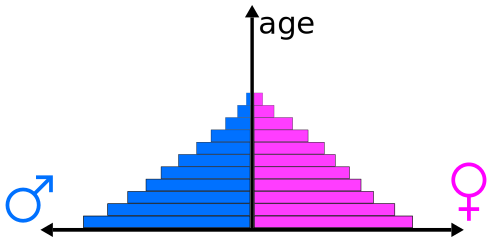
\includegraphics{images/Population_pyramid_example} 

}

\caption{Schematic diagram of a population pyramid (source: Wikipedia)}\label{fig:poppyramid}
\end{figure}

Here we look at the population counts for three countries: Germany,
Mexico and the US from the year 2000. You should have access to three
files: ``Germanypop.csv'', ``Mexicopop.csv'' and ``USpop.csv'', each
with the following columns:

\begin{itemize}
\tightlist
\item
  \textbf{male}: Population counts for males (\(\times\) 1000);
\item
  \textbf{female}: Population counts for females (\(\times\) 1000).
\end{itemize}

Each row corresponds to an age class, in the order: 0--4, 5--9, 10--14,
15--19, 20--24, 25--29, 30--34, 35--39, 40--44, 45--49, 50--54, 55--59,
60--64, 65--69, 70--74 and 75--79. Mexico then has a final age class of
80+; Germany has final age classes of 80--84 and 85+; and the US has
final age classes of 80--84, 85--89, 90--94 and 95+.

Original source: \href{http://www.census.gov/}{US Census}

(I downloaded these data sets from the very excellent QELP website:
\url{http://www.seattlecentral.edu/qelp/sets/032/032.html}, and wish to
thank the authors for providing a brilliant resource for teaching
statistics.)

In this exercise we will load these data into R, wrangle them into a
useful format and then produce a population pyramid using
\texttt{ggplot2}. We will aim to do all of this using a
\texttt{tidyverse} workflow where possible.

\subsection{Data Wrangling}\label{data-wrangling-1}

Firstly, we read the three data files into R, storing them as
\texttt{tibble} objects called \texttt{germany}, \texttt{mexico} and
\texttt{us}.

\begin{Shaded}
\begin{Highlighting}[]
\NormalTok{## read German data in}
\NormalTok{germany <-}\StringTok{ }\KeywordTok{read_csv}\NormalTok{(}\StringTok{"Germanypop.csv"}\NormalTok{)}

\NormalTok{## read Mexican data in}
\NormalTok{mexico <-}\StringTok{ }\KeywordTok{read_csv}\NormalTok{(}\StringTok{"Mexicopop.csv"}\NormalTok{)}

\NormalTok{## read US data in}
\NormalTok{us <-}\StringTok{ }\KeywordTok{read_csv}\NormalTok{(}\StringTok{"USpop.csv"}\NormalTok{)}
\end{Highlighting}
\end{Shaded}

We now need to bind these data sets together. One issue is that these
three data sets have different age classes. If we want to join the
tables together, we need to set consistent groupings in each data set.
For this we will set the maximum age class for each country to be
\texttt{"80+"}. Hence for Mexico we do not need to do anything, but for
Germany and the US we will need to group together the latter categories.

Let's do the US first.

\begin{Shaded}
\begin{Highlighting}[]
\NormalTok{us <-}\StringTok{ }\NormalTok{us %>%}
\StringTok{    }\KeywordTok{mutate}\NormalTok{(}\DataTypeTok{age =} \KeywordTok{ifelse}\NormalTok{(age ==}\StringTok{ "80-84"}\NormalTok{, }\StringTok{"80+"}\NormalTok{, age)) %>%}
\StringTok{    }\KeywordTok{mutate}\NormalTok{(}\DataTypeTok{age =} \KeywordTok{ifelse}\NormalTok{(age ==}\StringTok{ "85-89"}\NormalTok{, }\StringTok{"80+"}\NormalTok{, age)) %>%}
\StringTok{    }\KeywordTok{mutate}\NormalTok{(}\DataTypeTok{age =} \KeywordTok{ifelse}\NormalTok{(age ==}\StringTok{ "90-94"}\NormalTok{, }\StringTok{"80+"}\NormalTok{, age)) %>%}
\StringTok{    }\KeywordTok{mutate}\NormalTok{(}\DataTypeTok{age =} \KeywordTok{ifelse}\NormalTok{(age ==}\StringTok{ "95+"}\NormalTok{, }\StringTok{"80+"}\NormalTok{, age)) %>%}
\StringTok{    }\KeywordTok{group_by}\NormalTok{(age) %>%}
\StringTok{    }\KeywordTok{summarise}\NormalTok{(}\DataTypeTok{male =} \KeywordTok{sum}\NormalTok{(male), }\DataTypeTok{female =} \KeywordTok{sum}\NormalTok{(female))}
\end{Highlighting}
\end{Shaded}

\hypertarget{tsk23}{}\bblockT{23}

Go through the code above and understand what each line is doing. Repeat
this task for \texttt{germany}. \eblockT

\hyperlink{sol23}{\buttonS{Show Solution}}

We will now join the three data sets together on the \texttt{age}
column, before gathering together the \texttt{male} and \texttt{female}
counts for each country into two columns: one of population counts
(\texttt{pop}) and one relating to \texttt{sex} (which actually captures
\texttt{sex} and \texttt{country} at this stage). We will then separate
the \texttt{sex} and \texttt{country} values into two separate columns.
We do this using a single piped workflow that avoids us having to create
lots of temporary objects.

However, we must be careful here since the age classes do not match.
Hence we want to retain rows that don't match

\begin{Shaded}
\begin{Highlighting}[]
\NormalTok{pop <-}\StringTok{ }\NormalTok{germany %>%}
\StringTok{        }\KeywordTok{inner_join}\NormalTok{(mexico, }\StringTok{"age"}\NormalTok{, }\DataTypeTok{suffix =} \KeywordTok{c}\NormalTok{(}\StringTok{"_Germany"}\NormalTok{, }\StringTok{"_Mexico"}\NormalTok{)) %>%}
\StringTok{        }\KeywordTok{inner_join}\NormalTok{(us, }\StringTok{"age"}\NormalTok{) %>%}
\StringTok{        }\KeywordTok{rename}\NormalTok{(}\DataTypeTok{male_US =} \NormalTok{male, }\DataTypeTok{female_US =} \NormalTok{female) %>%}
\StringTok{        }\KeywordTok{gather}\NormalTok{(}\StringTok{"country"}\NormalTok{, }\StringTok{"pop"}\NormalTok{, -age) %>%}
\StringTok{        }\KeywordTok{separate}\NormalTok{(country, }\KeywordTok{c}\NormalTok{(}\StringTok{"sex"}\NormalTok{, }\StringTok{"country"}\NormalTok{), }\DataTypeTok{sep =} \StringTok{"_"}\NormalTok{) %>%}
\StringTok{        }\KeywordTok{mutate}\NormalTok{(}\DataTypeTok{country =} \KeywordTok{factor}\NormalTok{(country), }\DataTypeTok{sex =} \KeywordTok{factor}\NormalTok{(sex)) %>%}
\StringTok{        }\KeywordTok{mutate}\NormalTok{(}\DataTypeTok{age =} \KeywordTok{factor}\NormalTok{(age, }\DataTypeTok{levels =} \KeywordTok{unique}\NormalTok{(mexico$age)))}
\NormalTok{pop}
\end{Highlighting}
\end{Shaded}

\begin{verbatim}
## # A tibble: 102 x 4
##    age   sex   country   pop
##    <fct> <fct> <fct>   <int>
##  1 0-4   male  Germany  2055
##  2 10-14 male  Germany  2458
##  3 15-19 male  Germany  2404
##  4 20-24 male  Germany  2361
##  5 25-29 male  Germany  2623
##  6 30-34 male  Germany  3573
##  7 35-39 male  Germany  3756
##  8 40-44 male  Germany  3263
##  9 45-49 male  Germany  2883
## 10 50-54 male  Germany  2432
## # ... with 92 more rows
\end{verbatim}

\hypertarget{tsk24}{}\bblockT{24}

Go through the workflow above and understand what each line is doing and
why. Add comments to the code. If you don't understand, please ask one
of the demonstrators. \eblockT

\subsection{Visualisation}\label{visualisation}

Finally, we have wrangled our data into a useful form for data analysis.
Now we will try and plot some population pyramids using
\texttt{ggplot2}. We do this by tricking \texttt{ggplot} into plotting
stacked barplots, with \texttt{males} being plotted below the zero line,
and \texttt{females} above the zero line. We then flip the axes and use
faceting and colours to denote countries and sex respectively.

\begin{Shaded}
\begin{Highlighting}[]
\KeywordTok{ggplot}\NormalTok{(pop, }\KeywordTok{aes}\NormalTok{(}\DataTypeTok{x =} \NormalTok{age, }\DataTypeTok{y =} \KeywordTok{ifelse}\NormalTok{(sex ==}\StringTok{ "male"}\NormalTok{, -pop, pop), }\DataTypeTok{fill =} \NormalTok{sex)) +}\StringTok{ }
\StringTok{    }\KeywordTok{geom_bar}\NormalTok{(}\DataTypeTok{stat =} \StringTok{"identity"}\NormalTok{) +}
\StringTok{    }\KeywordTok{scale_y_continuous}\NormalTok{(}\DataTypeTok{breaks =} \KeywordTok{signif}\NormalTok{(}\KeywordTok{seq}\NormalTok{(-}\KeywordTok{max}\NormalTok{(pop$pop), }\KeywordTok{max}\NormalTok{(pop$pop), }\DataTypeTok{length.out =} \DecValTok{5}\NormalTok{), }\DecValTok{2}\NormalTok{), }
                     \DataTypeTok{labels =} \KeywordTok{abs}\NormalTok{(}\KeywordTok{signif}\NormalTok{(}\KeywordTok{seq}\NormalTok{(-}\KeywordTok{max}\NormalTok{(pop$pop), }\KeywordTok{max}\NormalTok{(pop$pop), }\DataTypeTok{length.out =} \DecValTok{5}\NormalTok{), }\DecValTok{2}\NormalTok{))) +}
\StringTok{    }\KeywordTok{coord_flip}\NormalTok{() +}
\StringTok{    }\KeywordTok{facet_wrap}\NormalTok{(~}\StringTok{ }\NormalTok{country, }\DataTypeTok{ncol =} \DecValTok{1}\NormalTok{) +}
\StringTok{    }\KeywordTok{ylab}\NormalTok{(}\StringTok{"Population counts (x1000)"}\NormalTok{) +}
\StringTok{    }\KeywordTok{xlab}\NormalTok{(}\StringTok{"Age (yrs)"}\NormalTok{) +}
\StringTok{    }\KeywordTok{guides}\NormalTok{(}\DataTypeTok{fill =} \KeywordTok{guide_legend}\NormalTok{(}\DataTypeTok{title =} \StringTok{"Sex"}\NormalTok{))}
\end{Highlighting}
\end{Shaded}

\begin{center}\includegraphics{_main_files/figure-latex/unnamed-chunk-131-1} \end{center}

Beautiful isn't it? (The horrendously stereotypical gender colours are
purely a coincidence due to the defaults in \texttt{ggplot2}, please
feel free to change them to something less egregious.) These plots are
hugely informative. We know that countries experiencing fast population
growth typically have a large number of individuals of reproductive age,
with a wider base to the pyramid. In contrast, populations that have
slow, static or even negative growth typically have more older
individuals; their pyramids tend to be wider at the top. We can also see
that the US has a much larger population than Mexico or Germany.

\subsection{Summarisation}\label{summarisation}

In the year 2000, the population distribution of Mexico shows a very
bottom-heavy pattern, suggesting few older people, but a large number of
young and middle-age people. In fact we can quantify this directly as:

\begin{Shaded}
\begin{Highlighting}[]
\NormalTok{pop %>%}
\StringTok{    }\KeywordTok{group_by}\NormalTok{(country, age) %>%}
\StringTok{    }\KeywordTok{summarise}\NormalTok{(}\DataTypeTok{pop =} \KeywordTok{sum}\NormalTok{(pop)) %>%}
\StringTok{    }\KeywordTok{arrange}\NormalTok{(country, age) %>%}
\StringTok{    }\KeywordTok{mutate}\NormalTok{(}\DataTypeTok{cumprop =} \KeywordTok{cumsum}\NormalTok{(pop /}\StringTok{ }\KeywordTok{sum}\NormalTok{(pop))) %>%}
\StringTok{    }\KeywordTok{select}\NormalTok{(-pop) %>%}
\StringTok{    }\KeywordTok{spread}\NormalTok{(age, cumprop)}
\end{Highlighting}
\end{Shaded}

\begin{verbatim}
## # A tibble: 3 x 18
## # Groups:   country [3]
##   country  `0-4`  `5-9` `10-14` `15-19` `20-24` `25-29` `30-34` `35-39`
## * <fct>    <dbl>  <dbl>   <dbl>   <dbl>   <dbl>   <dbl>   <dbl>   <dbl>
## 1 Germany 0.0483 0.0994   0.157   0.214   0.269   0.331   0.415   0.503
## 2 Mexico  0.114  0.227    0.338   0.445   0.545   0.637   0.713   0.777
## 3 US      0.0685 0.140    0.212   0.285   0.352   0.417   0.488   0.569
## # ... with 9 more variables: `40-44` <dbl>, `45-49` <dbl>, `50-54` <dbl>,
## #   `55-59` <dbl>, `60-64` <dbl>, `65-69` <dbl>, `70-74` <dbl>,
## #   `75-79` <dbl>, `80+` <dbl>
\end{verbatim}

\hypertarget{tsk25}{}\bblockT{25}

Go through the workflow above and understand what each line is doing and
why. Add comments to the code. If you don't understand, please ask one
of the demonstrators. Notice that we have used the \texttt{spread()}
function to produce a table that is \textbf{not} in `tidy' format, but
is better for visualising these specific outcomes. \eblockT

We can see here that around 55\% of Mexicans are younger than 25,
compared to around 27\% of Germans and 35\% of Americans. We can also
look at these figures split by sex:

\begin{Shaded}
\begin{Highlighting}[]
\NormalTok{pop %>%}
\StringTok{    }\KeywordTok{arrange}\NormalTok{(country, sex, age) %>%}
\StringTok{    }\KeywordTok{group_by}\NormalTok{(country, sex) %>%}
\StringTok{    }\KeywordTok{mutate}\NormalTok{(}\DataTypeTok{cumprop =} \KeywordTok{cumsum}\NormalTok{(pop /}\StringTok{ }\KeywordTok{sum}\NormalTok{(pop))) %>%}
\StringTok{    }\KeywordTok{select}\NormalTok{(-pop) %>%}
\StringTok{    }\KeywordTok{spread}\NormalTok{(age, cumprop)}
\end{Highlighting}
\end{Shaded}

\begin{verbatim}
## # A tibble: 6 x 19
## # Groups:   country, sex [6]
##   sex    country  `0-4`  `5-9` `10-14` `15-19` `20-24` `25-29` `30-34`
## * <fct>  <fct>    <dbl>  <dbl>   <dbl>   <dbl>   <dbl>   <dbl>   <dbl>
## 1 female Germany 0.0460 0.0946   0.150   0.203   0.257   0.315   0.395
## 2 female Mexico  0.110  0.219    0.327   0.430   0.529   0.619   0.698
## 3 female US      0.0655 0.134    0.203   0.272   0.336   0.400   0.471
## 4 male   Germany 0.0508 0.104    0.165   0.225   0.283   0.348   0.436
## 5 male   Mexico  0.118  0.235    0.350   0.460   0.562   0.654   0.729
## 6 male   US      0.0715 0.147    0.222   0.298   0.369   0.435   0.507
## # ... with 10 more variables: `35-39` <dbl>, `40-44` <dbl>, `45-49` <dbl>,
## #   `50-54` <dbl>, `55-59` <dbl>, `60-64` <dbl>, `65-69` <dbl>,
## #   `70-74` <dbl>, `75-79` <dbl>, `80+` <dbl>
\end{verbatim}

Mexico also has a very high proportion of young females: in fact 33\% of
the current population of women are of pre-reproductive age (0--14
years) and 49\% are of reproductive age (15--44). This means Mexico's
population is expected to rapidly increase in the near future. A general
pattern is that as countries transition from more agricultural economies
to more industrialised economies, birth rates drop (due to better access
to family planning, increased job opportunities for women, and various
other factors). As soon as birth rates approach death rates then
population growth declines, and the population pyramid becomes more
top-heavy. The US is currently classed as a medium-growth country, and
Germany a negative-growth country. The population pyramid plot also
helps visualise the overall differences in population sizes between the
three countries.

A good description of population demographics can be found in this short
video:

\begin{center}\includegraphics{images/population} \end{center}

Another great site on these sorts of topics is the
\href{https://ourworldindata.org/}{OurWorldInData} project.

\chapter{Epilogue}\label{epilogue}

These workshops have only really scratched the surface as to what can be
achieved using \texttt{tidyverse} and R. We haven't touched on the apply
functions included in the
\href{https://github.com/rstudio/cheatsheets/raw/master/purrr.pdf}{\texttt{purrr}}
package; we haven't looked at the utility of \textbf{list-columns}; or
began to explore the myriad other \texttt{ggplot2} geoms, such as
\texttt{geom\_violin()}, \texttt{geom\_bar()} or \texttt{geom\_hex()}.
We haven't looked at packages such as
\href{https://github.com/thomasp85/gganimate}{\texttt{gganimate}}, or
\href{https://plot.ly/r/}{\texttt{plotly}} for turning your R plots into
interactive HTML graphics, or the wonderful
\href{https://shiny.rstudio.com/gallery/}{\texttt{shiny}} package for
creating fully interactive websites, or the use of
\href{https://yihui.name/knitr/}{\texttt{knitr}} and
\href{https://rmarkdown.rstudio.com/}{\texttt{rmarkdown}} to produce
fully reproducible documents. In fact this workshop was written
completely in R using the
\href{https://bookdown.org/yihui/bookdown/}{\texttt{bookdown}} package,
by the inimitable \href{https://en.wikipedia.org/wiki/Yihui_Xie}{Yihui
Xie} (who also wrote \texttt{knitr}).

I hope that this workshop has helped to spark your interest in some of
the more powerful features of R. Please browse the myriad
\texttt{ggplot2} or \texttt{shiny} galleries for inspiration, and don't
hesitate to ask if you have any further questions.

\chapter{Answers}\label{answers}

\hypertarget{sol1}{} \bblockS{1}

Eloquent and inspiring solution.

\vspace{\baselineskip}

\hyperlink{tsk1}{\buttonT{Return to task}} \eblockS
\hypertarget{sol2}{} \bblockS{2}

\begin{Shaded}
\begin{Highlighting}[]
\KeywordTok{ggplot}\NormalTok{(iris) +}
\StringTok{    }\KeywordTok{geom_density}\NormalTok{(}\KeywordTok{aes}\NormalTok{(}\DataTypeTok{x =} \NormalTok{Sepal.Length, }\DataTypeTok{colour =} \NormalTok{Species))}
\end{Highlighting}
\end{Shaded}

\begin{center}\includegraphics{_main_files/figure-latex/unnamed-chunk-138-1} \end{center}

\vspace{\baselineskip}

\hyperlink{tsk2}{\buttonT{Return to task}} \eblockS
\hypertarget{sol3}{} \bblockS{3}

\begin{Shaded}
\begin{Highlighting}[]
\KeywordTok{ggplot}\NormalTok{(iris) +}
\StringTok{    }\KeywordTok{geom_density}\NormalTok{(}\KeywordTok{aes}\NormalTok{(}\DataTypeTok{x =} \NormalTok{Sepal.Length, }\DataTypeTok{fill =} \NormalTok{Species))}
\end{Highlighting}
\end{Shaded}

\begin{center}\includegraphics{_main_files/figure-latex/unnamed-chunk-139-1} \end{center}

We can see that now we have produced filled density plots. However,
since these overlap each other, it is difficult to see the full shapes
of these distributions.

\vspace{\baselineskip}

\hyperlink{tsk3}{\buttonT{Return to task}} \eblockS
\hypertarget{sol4}{} \bblockS{4}

\begin{Shaded}
\begin{Highlighting}[]
\KeywordTok{ggplot}\NormalTok{(iris) +}
\StringTok{    }\KeywordTok{geom_density}\NormalTok{(}\KeywordTok{aes}\NormalTok{(}\DataTypeTok{x =} \NormalTok{Sepal.Length, }\DataTypeTok{fill =} \NormalTok{Species), }\DataTypeTok{alpha =} \FloatTok{0.5}\NormalTok{)}
\end{Highlighting}
\end{Shaded}

\begin{center}\includegraphics{_main_files/figure-latex/unnamed-chunk-140-1} \end{center}

Now we can better see the shapes of these distributions.

\vspace{\baselineskip}

\hyperlink{tsk4}{\buttonT{Return to task}} \eblockS
\hypertarget{sol5}{} \bblockS{5}

\begin{Shaded}
\begin{Highlighting}[]
\KeywordTok{ggplot}\NormalTok{(iris) +}
\StringTok{    }\KeywordTok{geom_density}\NormalTok{(}\KeywordTok{aes}\NormalTok{(}\DataTypeTok{x =} \NormalTok{Sepal.Length, }\DataTypeTok{fill =} \NormalTok{Species), }\DataTypeTok{alpha =} \FloatTok{0.5}\NormalTok{) +}\StringTok{ }
\StringTok{    }\KeywordTok{xlab}\NormalTok{(}\StringTok{"Sepal Length (cm)"}\NormalTok{) +}\StringTok{ }\KeywordTok{ylab}\NormalTok{(}\StringTok{"Density"}\NormalTok{) +}\StringTok{ }
\StringTok{    }\KeywordTok{ggtitle}\NormalTok{(}\StringTok{"Density plots of sepal length by species"}\NormalTok{)}
\end{Highlighting}
\end{Shaded}

\begin{center}\includegraphics{_main_files/figure-latex/unnamed-chunk-141-1} \end{center}

\vspace{\baselineskip}

\hyperlink{tsk5}{\buttonT{Return to task}} \eblockS
\hypertarget{sol6}{} \bblockS{6}

In this case you get an error:

\begin{Shaded}
\begin{Highlighting}[]
\KeywordTok{ggplot}\NormalTok{(iris) +}
\StringTok{    }\KeywordTok{geom_point}\NormalTok{(}\KeywordTok{aes}\NormalTok{(}\DataTypeTok{x =} \NormalTok{Sepal.Length, }\DataTypeTok{y =} \NormalTok{Sepal.Width), }\DataTypeTok{colour =} \NormalTok{Species)}
\end{Highlighting}
\end{Shaded}

\begin{verbatim}
## Error in layer(data = data, mapping = mapping, stat = stat, geom = GeomPoint, : object 'Species' not found
\end{verbatim}

This is because you are trying to set a generic \texttt{colour} using a
vector object \texttt{Species}. Since the \texttt{colour} option is not
part of the aesthetics, \texttt{ggplot()} does not know where to find
\texttt{Species}.

\vspace{\baselineskip}

\hyperlink{tsk6}{\buttonT{Return to task}} \eblockS
\hypertarget{sol7}{} \bblockS{7}

\begin{Shaded}
\begin{Highlighting}[]
\KeywordTok{ggplot}\NormalTok{(gapminder[gapminder$year ==}\StringTok{ }\DecValTok{1952}\NormalTok{, ], }
       \KeywordTok{aes}\NormalTok{(}\DataTypeTok{x =} \NormalTok{gdpPercap, }\DataTypeTok{y =} \NormalTok{lifeExp, }\DataTypeTok{size =} \NormalTok{pop, }\DataTypeTok{colour =} \NormalTok{continent)) +}
\StringTok{    }\KeywordTok{geom_point}\NormalTok{() }
\end{Highlighting}
\end{Shaded}

\begin{center}\includegraphics{_main_files/figure-latex/unnamed-chunk-144-1} \end{center}

\vspace{\baselineskip}

\hyperlink{tsk7}{\buttonT{Return to task}} \eblockS
\hypertarget{sol8}{} \bblockS{8}

\begin{Shaded}
\begin{Highlighting}[]
\KeywordTok{ggplot}\NormalTok{(gapminder[gapminder$year ==}\StringTok{ }\DecValTok{1952}\NormalTok{, ], }
       \KeywordTok{aes}\NormalTok{(}\DataTypeTok{x =} \KeywordTok{log10}\NormalTok{(gdpPercap), }\DataTypeTok{y =} \NormalTok{lifeExp, }\DataTypeTok{size =} \NormalTok{pop, }\DataTypeTok{colour =} \NormalTok{continent)) +}
\StringTok{    }\KeywordTok{geom_point}\NormalTok{() }
\end{Highlighting}
\end{Shaded}

\begin{center}\includegraphics{_main_files/figure-latex/unnamed-chunk-145-1} \end{center}

\begin{Shaded}
\begin{Highlighting}[]
\KeywordTok{ggplot}\NormalTok{(gapminder[gapminder$year ==}\StringTok{ }\DecValTok{1952}\NormalTok{, ], }
       \KeywordTok{aes}\NormalTok{(}\DataTypeTok{x =} \NormalTok{gdpPercap, }\DataTypeTok{y =} \NormalTok{lifeExp, }\DataTypeTok{size =} \NormalTok{pop, }\DataTypeTok{colour =} \NormalTok{continent)) +}
\StringTok{    }\KeywordTok{geom_point}\NormalTok{() +}\StringTok{ }\KeywordTok{scale_x_log10}\NormalTok{()}
\end{Highlighting}
\end{Shaded}

\begin{center}\includegraphics{_main_files/figure-latex/unnamed-chunk-146-1} \end{center}

The plots differ purely in the labels for the \(x\)-axis.

\vspace{\baselineskip}

\hyperlink{tsk8}{\buttonT{Return to task}} \eblockS
\hypertarget{sol9}{} \bblockS{9}

\begin{Shaded}
\begin{Highlighting}[]
\KeywordTok{ggplot}\NormalTok{(gapminder[gapminder$year ==}\StringTok{ }\DecValTok{1952}\NormalTok{, ],}
       \KeywordTok{aes}\NormalTok{(}\DataTypeTok{x =} \NormalTok{gdpPercap, }\DataTypeTok{fill =} \NormalTok{continent)) +}
\StringTok{    }\KeywordTok{geom_histogram}\NormalTok{() +}
\StringTok{    }\KeywordTok{scale_x_log10}\NormalTok{() +}
\StringTok{    }\KeywordTok{xlab}\NormalTok{(}\StringTok{"log10(GDP per capita)"}\NormalTok{) +}\StringTok{ }
\StringTok{    }\KeywordTok{ylab}\NormalTok{(}\StringTok{"Count"}\NormalTok{) +}
\StringTok{    }\KeywordTok{ggtitle}\NormalTok{(}\StringTok{"1952"}\NormalTok{) +}
\StringTok{    }\KeywordTok{guides}\NormalTok{(}\DataTypeTok{fill =} \KeywordTok{guide_legend}\NormalTok{(}\DataTypeTok{title =} \StringTok{"Continent"}\NormalTok{)) }
\end{Highlighting}
\end{Shaded}

\begin{verbatim}
## `stat_bin()` using `bins = 30`. Pick better value with `binwidth`.
\end{verbatim}

\begin{center}\includegraphics{_main_files/figure-latex/unnamed-chunk-147-1} \end{center}

\vspace{\baselineskip}

\hyperlink{tsk9}{\buttonT{Return to task}} \eblockS
\hypertarget{sol10}{} \bblockS{10}

\begin{Shaded}
\begin{Highlighting}[]
\NormalTok{plotGapminder_gg <-}\StringTok{ }\NormalTok{function(data, }\DataTypeTok{year =} \DecValTok{1952}\NormalTok{) \{}
    \NormalTok{p <-}\StringTok{ }\KeywordTok{ggplot}\NormalTok{(gapminder[gapminder$year ==}\StringTok{ }\NormalTok{year, ],}
       \KeywordTok{aes}\NormalTok{(}\DataTypeTok{x =} \NormalTok{gdpPercap, }\DataTypeTok{fill =} \NormalTok{continent)) +}
\StringTok{    }\KeywordTok{geom_histogram}\NormalTok{() +}
\StringTok{    }\KeywordTok{scale_x_log10}\NormalTok{() +}
\StringTok{    }\KeywordTok{xlab}\NormalTok{(}\StringTok{"log10(GDP per capita)"}\NormalTok{) +}\StringTok{ }
\StringTok{    }\KeywordTok{ylab}\NormalTok{(}\StringTok{"Count"}\NormalTok{) +}
\StringTok{    }\KeywordTok{ggtitle}\NormalTok{(year) +}
\StringTok{    }\KeywordTok{guides}\NormalTok{(}\DataTypeTok{fill =} \KeywordTok{guide_legend}\NormalTok{(}\DataTypeTok{title =} \StringTok{"Continent"}\NormalTok{))}
    \KeywordTok{print}\NormalTok{(p)}
\NormalTok{\}}
\NormalTok{for(i in }\KeywordTok{c}\NormalTok{(}\DecValTok{1952}\NormalTok{, }\DecValTok{1982}\NormalTok{, }\DecValTok{1992}\NormalTok{, }\DecValTok{2002}\NormalTok{)) \{}
    \KeywordTok{plotGapminder_gg}\NormalTok{(gapminder, i)}
\NormalTok{\}}
\end{Highlighting}
\end{Shaded}

\begin{verbatim}
## `stat_bin()` using `bins = 30`. Pick better value with `binwidth`.
\end{verbatim}

\begin{center}\includegraphics{_main_files/figure-latex/unnamed-chunk-148-1} \end{center}

\begin{verbatim}
## `stat_bin()` using `bins = 30`. Pick better value with `binwidth`.
\end{verbatim}

\begin{center}\includegraphics{_main_files/figure-latex/unnamed-chunk-148-2} \end{center}

\begin{verbatim}
## `stat_bin()` using `bins = 30`. Pick better value with `binwidth`.
\end{verbatim}

\begin{center}\includegraphics{_main_files/figure-latex/unnamed-chunk-148-3} \end{center}

\begin{verbatim}
## `stat_bin()` using `bins = 30`. Pick better value with `binwidth`.
\end{verbatim}

\begin{center}\includegraphics{_main_files/figure-latex/unnamed-chunk-148-4} \end{center}

\vspace{\baselineskip}

\hyperlink{tsk10}{\buttonT{Return to task}} \eblockS
\hypertarget{sol11}{} \bblockS{11}

\begin{Shaded}
\begin{Highlighting}[]
\KeywordTok{ggplot}\NormalTok{(gapminder[gapminder$year ==}\StringTok{ }\DecValTok{1952}\NormalTok{, ],}
       \KeywordTok{aes}\NormalTok{(}\DataTypeTok{x =} \NormalTok{gdpPercap)) +}
\StringTok{    }\KeywordTok{geom_histogram}\NormalTok{()  +}
\StringTok{    }\KeywordTok{scale_x_log10}\NormalTok{()  +}
\StringTok{    }\KeywordTok{facet_wrap}\NormalTok{(~}\StringTok{ }\NormalTok{continent)}
\end{Highlighting}
\end{Shaded}

\begin{center}\includegraphics{_main_files/figure-latex/unnamed-chunk-149-1} \end{center}

\vspace{\baselineskip}

\hyperlink{tsk11}{\buttonT{Return to task}} \eblockS
\hypertarget{sol12}{} \bblockS{12}

\begin{Shaded}
\begin{Highlighting}[]
\KeywordTok{ggplot}\NormalTok{(gapminder,}
       \KeywordTok{aes}\NormalTok{(}\DataTypeTok{x =} \NormalTok{gdpPercap, }\DataTypeTok{fill =} \NormalTok{continent)) +}
\StringTok{    }\KeywordTok{geom_histogram}\NormalTok{() +}
\StringTok{    }\KeywordTok{scale_x_log10}\NormalTok{() +}
\StringTok{    }\KeywordTok{facet_wrap}\NormalTok{(~}\StringTok{ }\NormalTok{year)}
\end{Highlighting}
\end{Shaded}

\begin{center}\includegraphics{_main_files/figure-latex/unnamed-chunk-150-1} \end{center}

Here the axis labels are difficult to read, due to the plot size, so
perhaps we could rotate them. A quick Google search came up with
\href{http://www.cookbook-r.com/Graphs/Axes_(ggplot2)/}{this} page from
the R Graphics Cookbook, so let's try:

\begin{Shaded}
\begin{Highlighting}[]
\KeywordTok{ggplot}\NormalTok{(gapminder,}
       \KeywordTok{aes}\NormalTok{(}\DataTypeTok{x =} \NormalTok{gdpPercap, }\DataTypeTok{fill =} \NormalTok{continent)) +}
\StringTok{    }\KeywordTok{geom_histogram}\NormalTok{() +}
\StringTok{    }\KeywordTok{scale_x_log10}\NormalTok{() +}
\StringTok{    }\KeywordTok{facet_wrap}\NormalTok{(~}\StringTok{ }\NormalTok{year) +}
\StringTok{    }\KeywordTok{theme}\NormalTok{(}\DataTypeTok{axis.text.x =} \KeywordTok{element_text}\NormalTok{(}\DataTypeTok{angle =} \DecValTok{90}\NormalTok{, }\DataTypeTok{vjust =} \FloatTok{0.5}\NormalTok{))}
\end{Highlighting}
\end{Shaded}

\begin{verbatim}
## `stat_bin()` using `bins = 30`. Pick better value with `binwidth`.
\end{verbatim}

\begin{center}\includegraphics{_main_files/figure-latex/unnamed-chunk-151-1} \end{center}

\vspace{\baselineskip}

\hyperlink{tsk12}{\buttonT{Return to task}} \eblockS
\hypertarget{sol13}{} \bblockS{13}

\begin{Shaded}
\begin{Highlighting}[]
\NormalTok{## load data}
\NormalTok{ff <-}\StringTok{ }\KeywordTok{readRDS}\NormalTok{(}\StringTok{"ff.rds"}\NormalTok{)}

\NormalTok{## produce summary plot}
\KeywordTok{ggplot}\NormalTok{(ff, }\KeywordTok{aes}\NormalTok{(}\DataTypeTok{y =} \NormalTok{longevity, }\DataTypeTok{x =} \NormalTok{thorax, }
               \DataTypeTok{linetype =} \NormalTok{type, }\DataTypeTok{shape =} \NormalTok{type)) +}
\StringTok{    }\KeywordTok{geom_point}\NormalTok{() +}
\StringTok{    }\KeywordTok{geom_smooth}\NormalTok{(}\DataTypeTok{method =} \NormalTok{lm, }\DataTypeTok{se =} \NormalTok{F) +}
\StringTok{    }\KeywordTok{facet_wrap}\NormalTok{(~}\StringTok{ }\NormalTok{partners) +}
\StringTok{    }\KeywordTok{guides}\NormalTok{(}\DataTypeTok{linetype =} \KeywordTok{guide_legend}\NormalTok{(}\DataTypeTok{title =} \StringTok{"Partner Type"}\NormalTok{)) +}
\StringTok{    }\KeywordTok{guides}\NormalTok{(}\DataTypeTok{shape =} \KeywordTok{guide_legend}\NormalTok{(}\DataTypeTok{title =} \StringTok{"Partner Type"}\NormalTok{)) +}
\StringTok{    }\KeywordTok{ylab}\NormalTok{(}\StringTok{"Longevity (days)"}\NormalTok{) +}
\StringTok{    }\KeywordTok{xlab}\NormalTok{(}\StringTok{"Thorax length (mm)"}\NormalTok{)}
\end{Highlighting}
\end{Shaded}

\begin{center}\includegraphics{_main_files/figure-latex/unnamed-chunk-153-1} \end{center}

\vspace{\baselineskip}

\hyperlink{tsk13}{\buttonT{Return to task}} \eblockS
\hypertarget{sol14}{} \bblockS{14}

Yes, this data set is tidy. Each row corresponds to an individual
observation, each column to a variable and each cell to a specific
value.

\vspace{\baselineskip}

\hyperlink{tsk14}{\buttonT{Return to task}} \eblockS
\hypertarget{sol15}{} \bblockS{15}

\begin{Shaded}
\begin{Highlighting}[]
\NormalTok{iris %>%}\StringTok{ }
\StringTok{    }\KeywordTok{group_by}\NormalTok{(Species) %>%}
\StringTok{    }\KeywordTok{summarise}\NormalTok{(}\DataTypeTok{mnL =} \KeywordTok{mean}\NormalTok{(Sepal.Length), }\DataTypeTok{varL =} \KeywordTok{var}\NormalTok{(Sepal.Length),}
              \DataTypeTok{mnW =} \KeywordTok{mean}\NormalTok{(Sepal.Width), }\DataTypeTok{varW =} \KeywordTok{var}\NormalTok{(Sepal.Width))}
\end{Highlighting}
\end{Shaded}

\begin{verbatim}
## # A tibble: 3 x 5
##   Species      mnL  varL   mnW   varW
##   <fct>      <dbl> <dbl> <dbl>  <dbl>
## 1 setosa      5.01 0.124  3.43 0.144 
## 2 versicolor  5.94 0.266  2.77 0.0985
## 3 virginica   6.59 0.404  2.97 0.104
\end{verbatim}

\vspace{\baselineskip}

\hyperlink{tsk15}{\buttonT{Return to task}} \eblockS
\hypertarget{sol16}{} \bblockS{16}

No, this data is not in `tidy' format. We can see that each row
corresponds to a different \texttt{country}, but each column corresponds
to a different \texttt{year}. For this to be `tidy', we would need one
column containing the \texttt{country}, one containing the
\texttt{year}, and a third containing the GDP for each country in each
year.

\vspace{\baselineskip}

\hyperlink{tsk16}{\buttonT{Return to task}} \eblockS
\hypertarget{sol17}{} \bblockS{17}

\begin{Shaded}
\begin{Highlighting}[]
\NormalTok{gp_income %>%}\StringTok{ }
\StringTok{    }\KeywordTok{group_by}\NormalTok{(year) %>%}
\StringTok{    }\KeywordTok{summarise}\NormalTok{(}\DataTypeTok{mn =} \KeywordTok{mean}\NormalTok{(gdp))}
\end{Highlighting}
\end{Shaded}

\begin{verbatim}
## # A tibble: 25 x 2
##     year     mn
##    <dbl>  <dbl>
##  1  1991 12557.
##  2  1992 12623.
##  3  1993 12656.
##  4  1994 12886.
##  5  1995 13172.
##  6  1996 13470.
##  7  1997 13949.
##  8  1998 14221.
##  9  1999 14442.
## 10  2000 14905.
## # ... with 15 more rows
\end{verbatim}

Notice that although \texttt{year} is a numerical variable, R can still
group by unique values here.

\vspace{\baselineskip}

\hyperlink{tsk17}{\buttonT{Return to task}} \eblockS
\hypertarget{sol18}{} \bblockS{18}

\begin{Shaded}
\begin{Highlighting}[]
\NormalTok{gp_hiv <-}\StringTok{ }\KeywordTok{read_csv}\NormalTok{(}\StringTok{"indicator hiv estimated prevalence% 15-49.csv"}\NormalTok{) %>%}
\StringTok{            }\KeywordTok{rename}\NormalTok{(}\DataTypeTok{country =} \StringTok{`}\DataTypeTok{Estimated HIV Prevalence% - (Ages 15-49)}\StringTok{`}\NormalTok{) %>%}
\StringTok{            }\KeywordTok{gather}\NormalTok{(year, prevalence, -country) %>%}
\StringTok{            }\KeywordTok{mutate}\NormalTok{(}\DataTypeTok{year =} \KeywordTok{as.numeric}\NormalTok{(year)) %>%}
\StringTok{            }\KeywordTok{filter}\NormalTok{(!}\KeywordTok{is.na}\NormalTok{(country)) %>%}
\StringTok{            }\KeywordTok{filter}\NormalTok{(!}\KeywordTok{is.na}\NormalTok{(prevalence)) %>%}
\StringTok{            }\KeywordTok{filter}\NormalTok{(year >}\StringTok{ }\DecValTok{1990}\NormalTok{) %>%}
\StringTok{            }\KeywordTok{mutate}\NormalTok{(}\DataTypeTok{prevalence =} \KeywordTok{as.numeric}\NormalTok{(prevalence))}
\end{Highlighting}
\end{Shaded}

\vspace{\baselineskip}

\hyperlink{tsk18}{\buttonT{Return to task}} \eblockS
\hypertarget{sol19}{} \bblockS{19}

\begin{Shaded}
\begin{Highlighting}[]
\NormalTok{gp_hiv %>%}
\StringTok{    }\KeywordTok{filter}\NormalTok{(country ==}\StringTok{ "Brazil"} \NormalTok{|}\StringTok{ }\NormalTok{country ==}\StringTok{ "Uganda"}\NormalTok{) %>%}
\StringTok{    }\KeywordTok{ggplot}\NormalTok{(}\KeywordTok{aes}\NormalTok{(}\DataTypeTok{x =} \NormalTok{year, }\DataTypeTok{y =} \NormalTok{prevalence, }\DataTypeTok{colour =} \NormalTok{country)) +}
\StringTok{        }\KeywordTok{geom_line}\NormalTok{() +}\StringTok{ }\KeywordTok{xlab}\NormalTok{(}\StringTok{"Year"}\NormalTok{) +}\StringTok{ }\KeywordTok{ylab}\NormalTok{(}\StringTok{"Prevalence"}\NormalTok{) +}
\StringTok{        }\KeywordTok{guides}\NormalTok{(}\DataTypeTok{colour =} \KeywordTok{guide_legend}\NormalTok{(}\DataTypeTok{title =} \StringTok{"Country"}\NormalTok{))}
\end{Highlighting}
\end{Shaded}

\begin{center}\includegraphics{_main_files/figure-latex/unnamed-chunk-157-1} \end{center}

\vspace{\baselineskip}

\hyperlink{tsk19}{\buttonT{Return to task}} \eblockS
\hypertarget{sol20}{} \bblockS{20}

\begin{Shaded}
\begin{Highlighting}[]
\NormalTok{## here is one solution using filtering, piping and faceting}
\NormalTok{gp %>%}
\StringTok{    }\KeywordTok{filter}\NormalTok{(year ==}\StringTok{ }\DecValTok{1991} \NormalTok{|}\StringTok{ }\NormalTok{year ==}\StringTok{ }\DecValTok{1997} \NormalTok{|}\StringTok{ }\NormalTok{year ==}\StringTok{ }\DecValTok{2005} \NormalTok{|}\StringTok{ }\NormalTok{year ==}\StringTok{ }\DecValTok{2011}\NormalTok{) %>%}
\StringTok{    }\KeywordTok{ggplot}\NormalTok{(}\KeywordTok{aes}\NormalTok{(}\DataTypeTok{x =} \NormalTok{gdp, }\DataTypeTok{y =} \NormalTok{prevalence)) +}
\StringTok{    }\KeywordTok{geom_point}\NormalTok{() +}\StringTok{ }
\StringTok{    }\KeywordTok{scale_x_log10}\NormalTok{() +}
\StringTok{    }\KeywordTok{xlab}\NormalTok{(}\StringTok{"log10(GDP per capita)"}\NormalTok{) +}
\StringTok{    }\KeywordTok{ylab}\NormalTok{(}\StringTok{"HIV prevalence in 15-49 year olds"}\NormalTok{) +}
\StringTok{    }\KeywordTok{facet_wrap}\NormalTok{(~year)}
\end{Highlighting}
\end{Shaded}

\begin{center}\includegraphics{_main_files/figure-latex/unnamed-chunk-158-1} \end{center}

\vspace{\baselineskip}

\hyperlink{tsk20}{\buttonT{Return to task}} \eblockS
\hypertarget{sol21}{} \bblockS{21}

\begin{Shaded}
\begin{Highlighting}[]
\NormalTok{## read in data}
\NormalTok{gp_pop <-}\StringTok{ }\KeywordTok{read_csv}\NormalTok{(}\StringTok{"indicator gapminder population.csv"}\NormalTok{) %>%}
\StringTok{                }\KeywordTok{gather}\NormalTok{(year, pop, -}\StringTok{`}\DataTypeTok{Total population}\StringTok{`}\NormalTok{) %>%}
\StringTok{                }\KeywordTok{rename}\NormalTok{(}\DataTypeTok{country =} \StringTok{`}\DataTypeTok{Total population}\StringTok{`}\NormalTok{) %>%}
\StringTok{                }\KeywordTok{mutate}\NormalTok{(}\DataTypeTok{year =} \KeywordTok{as.numeric}\NormalTok{(year)) %>%}
\StringTok{                }\KeywordTok{filter}\NormalTok{(!}\KeywordTok{is.na}\NormalTok{(country)) %>%}
\StringTok{                }\KeywordTok{filter}\NormalTok{(!}\KeywordTok{is.na}\NormalTok{(pop)) %>%}
\StringTok{                }\KeywordTok{filter}\NormalTok{(year >}\StringTok{ }\DecValTok{1990}\NormalTok{)}

\NormalTok{## check no population data are missing}
\NormalTok{## hence all rows of gp can be matched}
\KeywordTok{anti_join}\NormalTok{(gp, gp_pop, }\DataTypeTok{by =} \KeywordTok{c}\NormalTok{(}\StringTok{"year"}\NormalTok{, }\StringTok{"country"}\NormalTok{))}
\end{Highlighting}
\end{Shaded}

\begin{verbatim}
## # A tibble: 0 x 4
## # ... with 4 variables: country <chr>, year <dbl>, gdp <int>,
## #   prevalence <dbl>
\end{verbatim}

\begin{Shaded}
\begin{Highlighting}[]
\NormalTok{## join to gp table}
\NormalTok{gp <-}\StringTok{ }\KeywordTok{inner_join}\NormalTok{(gp, gp_pop, }\DataTypeTok{by =} \KeywordTok{c}\NormalTok{(}\StringTok{"year"}\NormalTok{, }\StringTok{"country"}\NormalTok{))}
\end{Highlighting}
\end{Shaded}

\vspace{\baselineskip}

\hyperlink{tsk21}{\buttonT{Return to task}} \eblockS
\hypertarget{sol22}{} \bblockS{22}

\begin{Shaded}
\begin{Highlighting}[]
\NormalTok{## here is one solution using filtering, piping and faceting}
\NormalTok{gp %>%}
\StringTok{    }\KeywordTok{mutate}\NormalTok{(}\DataTypeTok{year =} \KeywordTok{as.numeric}\NormalTok{(year)) %>%}
\StringTok{    }\KeywordTok{filter}\NormalTok{(year ==}\StringTok{ }\DecValTok{1991} \NormalTok{|}\StringTok{ }\NormalTok{year ==}\StringTok{ }\DecValTok{1997} \NormalTok{|}\StringTok{ }\NormalTok{year ==}\StringTok{ }\DecValTok{2005} \NormalTok{|}\StringTok{ }\NormalTok{year ==}\StringTok{ }\DecValTok{2011}\NormalTok{) %>%}
\StringTok{    }\KeywordTok{ggplot}\NormalTok{(}\KeywordTok{aes}\NormalTok{(}\DataTypeTok{x =} \NormalTok{gdp, }\DataTypeTok{y =} \NormalTok{prevalence, }\DataTypeTok{size =} \NormalTok{pop)) +}
\StringTok{    }\KeywordTok{geom_point}\NormalTok{() +}\StringTok{ }
\StringTok{    }\KeywordTok{scale_x_log10}\NormalTok{() +}
\StringTok{    }\KeywordTok{guides}\NormalTok{(}\DataTypeTok{size =} \KeywordTok{guide_legend}\NormalTok{(}\DataTypeTok{title =} \StringTok{"Population size"}\NormalTok{)) +}
\StringTok{    }\KeywordTok{xlab}\NormalTok{(}\StringTok{"log10(GDP per capita)"}\NormalTok{) +}
\StringTok{    }\KeywordTok{ylab}\NormalTok{(}\StringTok{"HIV prevalence in 15-49 year olds"}\NormalTok{) +}
\StringTok{    }\KeywordTok{facet_wrap}\NormalTok{(~year)}
\end{Highlighting}
\end{Shaded}

\begin{center}\includegraphics{_main_files/figure-latex/unnamed-chunk-160-1} \end{center}

\vspace{\baselineskip}

\hyperlink{tsk22}{\buttonT{Return to task}} \eblockS
\hypertarget{sol23}{} \bblockS{23}

\begin{Shaded}
\begin{Highlighting}[]
\NormalTok{germany <-}\StringTok{ }\NormalTok{germany %>%}
\StringTok{    }\KeywordTok{mutate}\NormalTok{(}\DataTypeTok{age =} \KeywordTok{ifelse}\NormalTok{(age ==}\StringTok{ "80-84"}\NormalTok{, }\StringTok{"80+"}\NormalTok{, age)) %>%}
\StringTok{    }\KeywordTok{mutate}\NormalTok{(}\DataTypeTok{age =} \KeywordTok{ifelse}\NormalTok{(age ==}\StringTok{ "85+"}\NormalTok{, }\StringTok{"80+"}\NormalTok{, age)) %>%}
\StringTok{    }\KeywordTok{group_by}\NormalTok{(age) %>%}
\StringTok{    }\KeywordTok{summarise}\NormalTok{(}\DataTypeTok{male =} \KeywordTok{sum}\NormalTok{(male), }\DataTypeTok{female =} \KeywordTok{sum}\NormalTok{(female))}
\end{Highlighting}
\end{Shaded}

\vspace{\baselineskip}

\hyperlink{tsk23}{\buttonT{Return to task}} \eblockS

\end{document}
